\documentclass[specialist,
               substylefile = ../spbu.rtx,
               subf,href,colorlinks=true, 12pt]{disser}

\usepackage[a4paper,
            mag=1000, includefoot,
            left=3cm, right=1.5cm, top=2cm, bottom=2cm, headsep=1cm, footskip=1cm]{geometry}
\usepackage[utf8]{inputenc}
\usepackage[T2A]{fontenc}
\usepackage[english,russian]{babel}
\ifpdf\usepackage{epstopdf}\fi
\pagestyle{plain}

% Точка с запятой в качестве разделителя между номерами цитирований
%\setcitestyle{semicolon}

% Использовать полужирное начертание для векторов
\let\vec=\mathbf

% Включать подсекции в оглавление
\setcounter{tocdepth}{1}

\graphicspath{{../media/}}

\usepackage[style=gost-numeric]{biblatex}
\addbibresource{../biblio-u.bib}

\ifpdf\usepackage{epstopdf}\fi

\usepackage{multirow}
\usepackage{enumitem}
\usepackage{xcolor}
\usepackage{calc}

\newcounter{desccount}
\newcommand{\descitem}[2]{%
  \item[#1] \refstepcounter{desccount}\label{#2}
}
\newcommand{\descref}[1]{\hyperref[#1]{#1}}

\usepackage[ruled,vlined]{algorithm2e}

\usepackage[intlimits]{amsmath}
\usepackage{amsfonts}
\usepackage{amssymb}
\usepackage{amsthm}
\usepackage{mathrsfs}
\usepackage{mathtools}

\usepackage{hyperref}
\newtheorem{theorem}{Теорема}
\newcommand{\E}{\mathrm{E}}
\newcommand{\vfi}{\varphi}
\newcommand{\eps}{\varepsilon}
\newcommand{\prob}[1]{\mathrm{P}\left(#1\right)}
\newcommand{\R}{\ensuremath{\mathbb{R}}}
\newcommand{\Tau}{\ensuremath{\mathcal{T}}}
\newcommand{\GothB}{\mathfrak{B}}
\newcommand{\norm}[1]{\left\lVert#1\right\rVert}
\newcommand{\abs}[1]{\left\lvert#1\right\rvert}
\newcommand{\Vhat}{\hat{V}}
\newcommand{\vhat}{\hat{v}}
\newcommand{\maxset}[1]{\max\left\lbrace#1\right\rbrace}
\newcommand{\deltat}{\Delta t}
\DeclareMathOperator{\correlation}{cor}
\newcommand{\corr}[2]{\correlation\left(#1, #2\right)}
\DeclareMathOperator*{\argmax}{arg\,max}
\DeclareMathOperator*{\argmin}{arg\,min}
\DeclareMathOperator{\dd}{d}

%----------------------------------------------------------------
\begin{document}

%
% Титульный лист на русском языке
%

% Название организации
\institution{%
    Санкт-Петербургский государственный университет \\
    Прикладная математика и информатика \\
    Статистическое моделирование
}

\title{Выпускная квалификационная работа}

% Имя лица, допускающего к защите (зав. кафедрой)
% \apname{д.\,ф.-м.\,н., профессор С.\,М.~Ермаков}

% Тема
\topic{\normalfont\scshape%
    Имитационная модель американского опциона}

% Автор
\author{Миллер Анастасия Александровна}

% Научный руководитель
\sa       {С.\,М.~Ермаков}
\sastatus {д.\,ф.-м.\,н., профессор}

% Рецензент
\rev      {А.\,В.~Дмитриев}
\revstatus{нач.\,лаб.}

% Город и год
\city{Санкт-Петербург}
\date{\number\year}

\maketitle

%%
%% Titlepage in English
%%
%
\institution{%
    Saint Petersburg State University \\
    Applied Mathematics and Computer Science \\
    Statistical Modelling
}
%
\title{Graduation Project}
%
%% Topic
\topic{\normalfont\scshape %
    Simulation model of American option}
%
%% Author
\author{Miller Anastasiia} % Full Name
%
%% Scientific Advisor
\sa       {S.\,M.~Ermakov}
\sastatus {Professor}
%
%% Reviewer
\rev      {A.\,V.~Dmitriev}
\revstatus{Head of the Lab}
%
%% City & Year
\city{Saint Petersburg}
\date{\number\year}
%
\maketitle[en]

\pagestyle{footcenter}
\chapterpagestyle{footcenter}

\tableofcontents

%!TEX root = thesis.tex
\intro
В работе рассмотрены основные подходы к оценке стоимости Американских опционов и приведено их сравнение между собой (как теоретическое, так и на численных примерах). Основной целью работы было исследование вопроса о применении метода квази Монте-Карло к задаче оценки стоимости Американского опциона.

Ниже в этом разделе разобрано понятие опциона (секция \ref{sec:intro:option_definition}) и описана формальная постановка задачи нахождения стоимости Американского опциона (секция \ref{sec:intro:option_price}). В главе \ref{cha:classic_approaches_to_option_pricing} приведены основные способы оценки этой стоимости. В главе \ref{cha:QMC_for_variance_reduction} даны основные сведения о методе квази Монте-Карло и рассмотрены особенности этого метода в приложении к финансовым задачам (в частности --- задаче оценки стоимости Американского опциона). В главе \ref{cha:tree_pruning_for_american_option} предложен новый подход к оценке стоимости Американского опциона, основывающийся на идее <<прореживания>> дерева состояний случайного процесса. Глава \ref{cha:numerical_results} содержит результаты численных экспериментов, подтверждающих или опровергающих высказанные в предыдущих главах гипотезы.
% В главе \ref{cha:classic_approaches_to_option_pricing} описана задача оценки Американских опционов (в секции \ref{sec:option_price}) и приведены основные методы её решения (случайные деревья, стохастические сетки и линейная регрессия, раздел \ref{sec:estimators}). 
% Глава \ref{cha:variance_reduction} содержит описание методов снижения дисперсии оценок, в частности, применение квази Монте-Карло. 
% В главе \ref{cha:quasi_monte_carlo} более подробно разобрана теория квази Монте-Карло и приведены обоснования для выбора размерности квазислучайной последовательности. В большинстве секций теоретические сведения подкреплены демонстрацией вычислений на конкретных примерах.

\section{Понятие опциона} % (fold)
\label{sec:intro:option_definition}

Опцион --- это широко распространённый вторичный (производный) финансовый инструмент. Опцион является контрактом между продавцом опциона и покупателем опциона о том, что покупатель имеет право, но не обязательство, купить (в случае опциона на покупку, call option) или продать (в случае опциона на продажу, put option) указанный в контракте базовый актив по заранее оговорённой цене (\emph{цене страйк}) в определённый контрактом момент в будущем или на протяжении определённого отрезка времени. Продавца опциона контракт обязует совершить ответную продажу (для опциона на покупку) или покупку (для опциона на продажу) в случае, если покупатель пожелает исполнить своё право. Реализация такой сделки называется \emph{исполнением опциона}.

Различают опционы европейского и американского типа. Опцион европейского типа выписывается на фиксированный момент времени в будущем, опцион американского типа --- на отрезок времени. Промежуточный вариант, когда опцион может быть исполнен только в определённые даты (например, в конце каждого квартала в течение года), часто называют Бермудским опционом.

Исполнение опциона может быть выгодно его владельцу (когда цена базового актива в контракте ниже текущей рыночной в случае опциона на покупку, когда цена базового актива выше текущей рыночной в случае опциона на продаже), поэтому опционный контракт сам по себе тоже имеет стоимость. Ищется стоимость опциона в модели эффективного рынка, то есть такая цена $V$, при которой ни продавец, ни покупатель опциона в среднем не получают прибыли.

% section intro:option_definition (end)

\section{Стоимость Американского опциона как случайная величина} % (fold)
\label{sec:intro:option_price}

В случае опциона европейского типа существует решение в замкнутой форме (модель Блэка-Шоулса \cite{Black1973} и её усовершенствования). Оценка Американского опциона является более сложной задачей.

Опцион определяется 
\begin{itemize}[noitemsep,topsep=0pt]
\item своим временем жизни $[0;T]$, 
\item базовым активом $X$ (под $X(t)$ будем подразумевать состояние актива в момент времени $t$, являющееся случайной величиной, под $S(t) = S(X(t))$ --- цену базового актива в момент $t$), на который выписан опцион (список возможных активов на территории Российской Федерации представлен в \cite{fsfr}), 
\item процессом $U(t),\;t\in{[0;T]}$, представляющим дисконтированное значение функции выплат (разницы между рыночной стоимостью базового актива и ценой страйк, оговорённой в контракте; значение функции выплат показывает выгоду, получаемую владельцем опциона при исполнении),
\item множеством $\Tau$ моментов времени, в которых возможно исполнить опцион.
\end{itemize} 
Будем также считать, что существует $h_t: U(t) = h_t\left(X(t)\right)$. Тогда для Американского опциона с функцией выплат $h_t\left(X_t\right)$ нахождение цены $V$ --- это задача оптимальной остановки (optimal stopping problem):
\begin{equation}\label{eq:optimal_stopping}
V = \max_{\tau} \E h_\tau\left(X_\tau\right).
\end{equation}

При дискретизации \eqref{eq:optimal_stopping} (принятии предположения о том, что $\Tau$ -- конечное множество $\left\lbrace t_i\right\rbrace_{i=0}^n \in \left[0;T\right], t_0 = 0, t_n = T$) задача обретает эквивалентную формулировку о нахождении $V_0\left(X_0\right)$ в системе
\begin{equation}\label{eq:option-recursive}\begin{aligned}
            V_m\left(x\right) &= h_m\left(x\right), \\
            V_{i-1}\left(x\right) &= \maxset{h_{i-1}\left(x\right),\E\left[V_i\left(X_i\right)|X_{i-1}=x\right]}.
\end{aligned}\end{equation}
Здесь $\forall i \in{0\mathbin{:}n}\quad h_i = h_{t_i}$, и такие обозначения будут использоваться и далее в тексте.

Далее в работе в основном будет использоваться формулировка \eqref{eq:option-recursive}. 

% section intro:option_price (end)
%!TEX root = thesis.tex
\chapter{Классические методы оценки стоимости Американского опциона} % (fold)
\label{cha:classic_approaches_to_option_pricing}

Cамый наивный способ оценить стоимость Американского опциона --- это промоделировать множество возможных траекторий базового актива, посчитать максимальную выплату по опциону в каждом из этих случаев (как максимум из значений $h_t(X_t)$ на промоделированной траектории $\left\{ X_t \right\}_{t \in \Tau}$) и усреднить результаты по всем промоделированным траекториям. Это классический метод Монте-Карло. Как будет видно далее (в разделе \ref{sec:results:classical_approaches}), дисперсия наивного Монте-Карло для этой задачи слишком велика.

Все рассмотренные далее способы --- это различные попытки уменьшить дисперсию наивного варианта путём увеличения числа моделируемых траекторий. 

\section{Случайные деревья} % (fold)
\label{sec:classic_approaches:tree_estimator}

Метод случайного дерева основан на моделировании цепи $X_0, X_1, \ldots X_n$ состояний актива. Зафиксируем параметр ветвления $b$. Из исходного состояния $X_0$ смоделируем $b$ независимых между собой следующих состояний $X_1^1, X_1^2, \ldots X_1^b$, все с условием $X_0$. Для каждого $X_1^i$ снова смоделируем $b$ независимых между собой последующих состояний $X_2^{i1}, \ldots X_2^{ib}$. На $m$-ом шаге будем иметь $b^m$ состояний, и это и есть источник основного недостатка этого метода --- времени работы порядка $O(b^m)$. Схема приведена на рис.\,\ref{fig:exponential_tree}.
\begin{figure}[b]
    \centering
    \includegraphics{exponential_tree.pdf}
    \caption{Случайное дерево для $b = 3$ и $m = 2$}
    \label{fig:exponential_tree}
\end{figure}

В \cite{Broadie1997} предложены оценки для $V_0\left(X_0\right)$ сверху ($\hat{V}_0$) и снизу ($\hat{v}_0$):
\begin{equation}\label{eq:upper}
\begin{aligned}
    \hat{V}_m^{j_1 \ldots j_m} &= h_m\left(X_m^{j_1 \ldots j_m}\right), \\
    \hat{V}_i^{j_1 \ldots j_i} &= \max \left\lbrace h_i \left( X_i^{j_1 \ldots j_i} \right), \frac{1}{b} \sum_{j = 1}^b \hat{V}_{i+1}^{j_1 \ldots j_i j}\right\rbrace,
\end{aligned}\end{equation}
\begin{equation}\label{eq:lower}
\begin{aligned}
    \hat{v}_m^{j_1 j_2 \cdots j_m} &= h\left( X_m^{j_1 j_2 \cdots j_m}\right), \\
    \hat{v}_{ik}^{j_1 j_2 \cdots j_i} &= \left\lbrace
                \begin{array}{l l}
                    h\left( X_i^{j_1 j_2 \cdots j_i}\right), & \, \text{если } \frac{1}{b-1}\sum_{j=1, j\not= k}^b \hat{v}_{i+1}^{j_1 j_2 \cdots j_i j} \leq h\left(X_i^{j_1 j_2 \cdots j_i}\right), \\
                    \hat{v}_{i+1}^{j_1 j_2 \cdots j_i k}, & \, \text{иначе}
                \end{array}\right. \\
    \hat{v}_i^{j_1 j_2 \cdots j_i} &= \frac{1}{b}\sum_{k=1}^b \hat{v}_{ik}^{j_1 j_2 \cdots j_i}.
\end{aligned}\end{equation}

В этой же работе доказаны их состоятельность, смещённость и асимптотическая несмещённость. Так, если $\exists\: p' > 1: \forall t \in \Tau \quad \E\left[ \abs{h_t(X_t)}^{p'} \right] < \infty$, то $\forall p \in \left(0; p'\right)$ имеет место сходимость по вероятности $\Vhat_0(b) \overset{\mathcal L^p}{\to} V_0$. Следовательно, $\E\Vhat_0(b) \underset{b \to\infty}{\longrightarrow} V_0$. При этом $\forall b \in \mathbb N \quad \E\Vhat_0(b) \geq V_0$.

Алгоритм прост в реализации и нетребователен по памяти: при реализации обходом в глубину память ограничена $O(m)$. Основной недостаток --- экспоненциальная сложность по времени: обойти всё дерево получится за $O(m^b)$.

% section tree_estimator (end)

\section{Стохастические сетки} % (fold)
\label{sec:classic_approaches:mesh_estimator}

Метод стохастической сетки \cite{Broadie2004,Kashtanov2015} также предлагает оценки сверху и снизу для решения \eqref{eq:option-recursive}, но принцип построения оценок несколько отличается от рассмотренного выше метода случайного дерева.

Из начального состояния $X_0$ для оценки опциона с $m$ моментами исполнения, равноотстоящими во времени от 0 до $T$, зададим сетку $X_n^i,\; n\in 1\mathbin{:}m,\, i \in 1\mathbin{:}b$, узлы которой --- реализации случайной величины с плотностью $p_{0, n}(X_0, \cdot)$ (маргинальные плотности; также рассматриваются средние плотности), а $p_{k, n}(x, y) = \prob{X_n = y \middle\vert X_k = x}$. Тогда определяются $\rho_{n, j}(x, y) = p_{n-1, n}(x, y) / p_{0, n}(X_0, y)$, сокращения $\rho_{n, j}(i, j) = \rho_{n, j}(X_{n-1}^i, X_n^j)$ и оценка в каждом узле сетки
\begin{equation}\label{eq:mesh_estimator}
\hat Y_n(i) = \max\left\lbrace h_n(i), \frac{\sum_j \rho_{n+1}(i, j) \hat Y_{n+1}(j)}{\sum_j \rho_{n+1}(i, j)} \right\rbrace.
\end{equation}
Под знаком $\max$ в \eqref{eq:mesh_estimator} стоят выручка, которую можно получить, если исполнить опцион в момент $n$ ($h_n(i)$), и оценка ожидаемой выручки $\E\left[V_i\left(X_i\right)|X_{i-1}=x\right]$: выражение $\left(\sum_j \rho_{n+1}(i, j) \hat Y_{n+1}(j)\right) / \left(\sum_j \rho_{n+1}(i, j)\right)$ можно рассматривать как оценку математического ожидания с помощью непараметрический регрессии.

Иллюстрация взаимоотношений между узлами сетки приведена на рис.,\ref{fig:stochastic_mesh}. Тогда оценка справедливой стоимости опциона --- это $$\hat Y_0 = \max\left\lbrace h_0(X_0), \frac{\sum_j \rho_{1}(X_0, X_1^j) \hat Y_{1}(X_1^j)}{\sum_j \rho_{1}(X_0, X_1^j)} \right\rbrace.$$

\begin{figure}[t]
    \centering
    \includegraphics{stohastic_mesh_vector.eps}
    \caption{Стохастическая сетка для $b = 5$ и $m = 3$}
    \label{fig:stochastic_mesh}
\end{figure}

Этот метод работает гораздо быстрее, чем метод случайных деревьев: сложность и по времени, и по памяти составляет $O(mb)$. Недостатком являются трудоёмкие вычисления в многомерном случае: в отличие от случайного дерева, для обсчёта которого нужно лишь уметь вычислить $h_t(X_t)$ (для традиционного примера максимум-опциона на покупку $h_t(X_t) = \left(\max(X_t) - K\right)^+$, если $X_t$ -- вектор стоимостей базовых активов в момент $t$), для стохастических сеток нужно точно вычислять $\rho_n(i, j)$.

% section mesh_estimator (end)

\section{Метод наименьших квадратов} % (fold)
\label{sec:classic_approaches:least_squares}

Несколько отличающийся от двух предыдущих вариант --- метод оценки с помощью линейной регрессии \cite{Longstaff2001}. Согласно формулировке \eqref{eq:option-recursive}, в каждый момент $t$ мы хотим знать математическое ожидание стоимости удержания (неисполнения) опциона при условии его текущего состояния. Классический инструмент для оценки условного математического ожидания --- это линейная регрессия. Будем оценивать стоимость удержания опциона следующим образом:

\begin{equation}\label{eq:lsm_continuation}
\E\left(V_i(X_i)\middle\vert X_{i-1} = x\right) \approx \sum_{r=1}^M \beta_{ir} \psi_r(x) = \beta_i^\mathsf{T}\psi(x).
\end{equation}
Здесь $\psi(x) = \left(\psi_1(x), \dots, \psi_M(x)\right)^\mathsf{T}$ --- это набор регрессоров, используемых для построения оценки. В оригинальной статье использовались полиномы Лагера (\cite[секция~2.2 на стр.~122]{Longstaff2001}) и для построения регрессии использовались только те траектории, на которых опцион в $i-1$-й момент времени находился в деньгах.

Используемая здесь сетка похожа на ту, что была в методе стохастической сетки: моделируем несколько траекторий, тем самым получая нужный набор примеров (см. рис.,\ref{fig:least_squares}). Коэффициенты $\beta$ оцениваются по методу наименьших квадратов. 

\begin{figure}[t]
    \centering
    \includegraphics{stohastic_mesh_vector_phase_0.eps}
    \caption{Стохастическая сетка для метода наименьших квадратов, $b = 5$ и $m = 3$}
    \label{fig:least_squares}
\end{figure}

Для каждого узла сетки теперь возможно оценить стоимость удержания опциона по выражению \eqref{eq:lsm_continuation} и понять, было бы оптимальным решением исполнить опцион в этот момент (если выручка от немедленного исполнения превосходит стоимость удержания опциона, то оптимальным решением будет исполнить опцион, иначе -- оставить его для исполнения в какой-либо из последующих моментов). После того, как установлены моменты оптимального исполнения опциона для каждой из исходных траекторий, составлявших сетку, стоимость опциона на траектории устанавливается равной выплате, полученной в оптимальный для этой траектории момент исполнения. Итоговая стоимость опциона оценивается усреднением по всем траекториям. Более формально эта процедура изложена в алгоритме~\ref{alg:least_squares_estimation}.

\begin{algorithm}[h]
    \SetAlgorithmName{Алгоритм}{алгоритм}{Список алгоритмов}
    \SetKwInput{KwData}{Входные данные}
    \SetKwInput{KwResult}{Результат}
    \SetKw{KwTo}{до}\SetKwFor{For}{Для}{\string:}{}%
    \KwData{сетка из $b$ промоделированных траекторий состояния базового актива $X_n^i,\;\;n\in 1\mathbin{:}m,\;i \in 1\mathbin{:}b$}
    \KwResult{$\Vhat$ -- оценка стоимости опциона}
    
    положим стоимость опциона равной выплате по нему в последний момент исполнения:\\$C_i \leftarrow h_{t_m}\left(X_m^i\right)$, $C = \left(C_1, \dots, C_b\right)^{\mathsf T}$\;
    \For{$n\leftarrow m-1$ \KwTo $1$}{
        % дисконтируем стоимость опциона: $C \leftarrow e^{-r\deltat} \cdot C$\tcc*[r]{если $h_t$ уже дисконтированная, этого делать не нужно}\;
        $X_i \leftarrow S_n^i$, $X = \left(X_1, \dots, X_b\right)^{\mathsf T}$\;
        выплаты по исполнении опциона $P_i \leftarrow h_{t_n}\left(X_n^i\right)$, $P = \left(P_1, \dots, P_b\right)^{\mathsf T}$\;
        строим линейную регрессию $C$ на $X$ через набор базисных функций $\psi$ по всем тем примерам, где опцион в деньгах:\\ $\beta \leftarrow \argmin_{\beta'\in\R^M} \norm{\left({\beta'}^\mathsf{T}\psi(X_i) - C_i\right)_{\left\{i \middle\vert P_i > 0\right\}}}^2$\;
        стоимость удержания опциона $H_i = \beta^\mathsf{T}\psi(X_i)$\;
        \For{всех $i$ таких, что $P_i > H_i$}{
            $C_i \leftarrow P_i$\;
        }
    }
    $\Vhat \leftarrow \frac{1}{b}\sum_{i=1}^b C_i$

    \caption{Оценка стоимости опциона по методу наименьших квадратов}
\label{alg:least_squares_estimation}
\end{algorithm}

В \cite{Glasserman2004} указано, что метод наименьших квадратов можно считать частным случаем метода стохастической сетки со специальным выбором весов. Тем не менее, часто эти подходы рассматриваются по отдельности.

В той же статье, где предложен этот метод, приводится доказательство того, что обсуждаемая оценка является состоятельной и несмещённой. Сформулируем это утверждение несколько точнее: оно понадобится в разделе\,\ref{sec:tree_pruning:consistency}.

Из формулировок (\ref{eq:optimal_stopping}, \ref{eq:option-recursive}) и предположения о марковости процесса следует, что функция $V_i\left(x\right)$ -- это стоимость опциона, который может быть исполнен в моменты $t_i, \dots, t_n$ и в момент $t_i$ имеет стоимость $x$. Тогда результат из \cite{Longstaff2001} можно сформулировать следующим образом:

\begin{theorem}
    Пусть $\E\left(V_i(X_i)\middle\vert X_{i-1} = x\right) = F(i-1, x)$ является $\mathcal L^2$-интегрируемой функцией. Тогда для набора базисных функций $\left\{\psi_i(x)\right\}_{i=1}^{\infty}$ имеет место разложение $$F(i-1, x) = \sum_{j=1}^\infty a_{i-1,j} \psi_j(x).$$
    Введём также $F_M(i-1, x) = \sum_{j=1}^M a_{i-1,j} \psi_j(x)$ и будем оценивать его с помощью дисконтированных значений $V_i\left(x\right)$ на тех траекториях, где опцион в момент $t_{i-1}$ находится в деньгах. Утверждается, что такая оценка $\widehat{F_M}(i-1, x)$ сходится к $F_M(i-1, x)$ при $N\to\infty$, где $N$ -- количество промоделированных траекторий, на которых опцион в момент $t_{i-1}$ находился в деньгах. Более того, $\widehat{F_M}(i-1, x)$ является лучшей линейной несмещённой оценкой по среднеквадратичной метрике.
\end{theorem}

% chapter classic_approaches_to_option_pricing (end)
%!TEX root = thesis.tex
\chapter{Применение Квази Монте-Карло для повышения точности оценок} % (fold)
\label{cha:QMC_for_variance_reduction}

Все методы, изложенные в главе \ref{cha:classic_approaches_to_option_pricing}, разработаны для того, чтобы за как можно меньшее время работы получить как можно более точную оценку для $V_0$. Получить меньшую дисперсию оценки (а, значит, более точную оценку) можно не только использованием более эффективного алгоритма, но и с помощью техник снижения дисперсии. 

Стандартные подходы к снижению дисперсии оценки по методу Монте-Карло используют случайную природу метода. Так, метод \emph{противоположных переменных} использует тот факт, что дисперсия суммы двух одинаково распределённых зависимых случайных величин $\xi$ и $\eta$ с отрицательной ковариацией $\mathrm{cov}\left(\xi, \eta\right) < 0$ равна 
$$\mathrm D\left(\xi + \eta\right) = \mathrm D \xi + 2 \mathrm{cov}\left(\xi, \eta\right) + \mathrm D\eta < 2 \mathrm D\eta.$$
Таким образом, использование в методе Монте-Карло вместо независимых одинаково распределённых случайных величин зависимых с отрицательной корреляцией позволяет снизить дисперсию оценки. Подробнее см.~\cite[раздел~4.2, стр.~205]{Glasserman2004}.

Метод \emph{контрольных переменных} также использует разложение дисперсии суммы двух случайных величин. Идея здесь состоит в том, что если взять две скоррелированных случайных величины $\xi$ и $\eta$, для одной из которых известно математическое ожидание (например, $\E\eta$), то на каждой реализации пары можно осуществлять коррекцию. Отклонение величины $\xi$ от $\E\xi$ похоже на отклонение $\eta$ от $\E\eta$; отсюда можно сконструировать скорректированную оценку $\bar\xi = \xi - b\left(\eta - \E\eta\right)$ и доказать, что при оптимальном $b$ $\mathrm D \bar\xi / \mathrm D\xi = 1 - \corr{\xi}{\eta}$. Подробнее см.~\cite[раздел~4.1, стр.~185]{Glasserman2004}.

Принципиально иной подход к снижению дисперсии появляется из области численного интегрирования. Математическое ожидание случайной величины, к которому стремится среднее множества её реализаций, является интегралом по носителю этой случайной величины (по определению математического ожидания). Поэтому метод Монте-Карло можно использовать для вычисления значения интегралов, и по той же причине его можно сравнивать с методами вычисления интеграла по регулярной сетке.

Метод квази Монте-Карло \cite{Chi2004} использует вместо последовательностей случайных точек детерминированные последовательности, обладающие свойством равномерно покрывать заданное пространство. Равномерность получаемой сетки и приводит к оценкам более точным, чем при использовании случайной сетки.

В этой главе изучаются особенности применения метода квази Монте-Карло для снижения дисперсии оценок в финансовых задачах (в частности, задаче оценки Американского опциона). В разделе~\ref{sec:qmc:qmc_definition} изложены основные сведения о квазислучайном методе: определение дискрепанса, неравенство Коксмы-Хлавки. В разделе~\ref{sec:qmc:randomization} описан метод рандомизации сдвигом, использующийся для получения более простых оценок погрешности квазислучайного метода, нежели неравенство Коксмы-Хлавки. Раздел~\ref{sec:qmc:monte_carlo_in_option_pricing} освещает основные вопросы, связанные с применением квази Монте-Карло к финансовым задачам. Для одного из этих вопросов решение известно, для второго в этом разделе предложено два варианта решения, которые сравниваются на численных экспериментах в разделе~\ref{sec:results:qmc_to_classical_methods}. %Также упомянуты более стандартные техники (метод противоположных переменных, метод контрольных переменных).

\section{Основные понятия} % (fold)
\label{sec:qmc:qmc_definition}

Отклонением (star discrepancy, $D^*$) последовательности из $N$ $d$-мерных случайных векторов в гиперкубе $\left[0;1\right]^d$ называют величину
$$D_N^* = D_N^*\left(X_1, \dots, X_N\right) = \sup_{v = (v_1, \dots, v_d) \in \left[0;1\right]^d} N \abs{\frac{\#\left\{ X_i \in J(v) \right\}}{N} - \prod_{j = 1}^d v_j},$$
где $J(v) = \left[0; v_1\right) \times \dots \times \left[0; v_d\right)$.

В случае, когда последовательность $\left\{ X_i\right\}_{i=1}^\infty$ такова, что $\forall N \: D_N^* \leq C_s \frac{(\ln N)^s}{N}$, последовательность называется последовательностью с низким отклонением (или с низким дискрепансом). С вычислительной точки зрения она представляет интерес из-за неравенства Коксмы-Хлавки: для интеграла, оцененного по этой последовательности, верно утверждение

\begin{equation}\label{eq:koksma-hlawka}
\abs{\int_{\left[0;1\right]^d} f(X) \dd X - \frac{1}{N}\sum_{i=1}^N f(X_i)} \leq \mathrm{Var}f\cdot \frac{D_N^*\left(X_1, \dots, X_N\right)}{N},
\end{equation}
где $\mathrm{Var}f$ -- вариация функции в смысле Харди-Краузе. Тогда при использовании последовательности с низким дискрепансом ошибка оценки интеграла имеет порядок $O\left(D_N^*\left(X_1, \dots, X_N\right)/N\right) = O\left((\ln N)^s / N^2\right)$. В случае обычного Монте-Карло размер отклонения оценки от математического ожидания имеет порядок $O(1 / \sqrt{N})$. Нетрудно заметить, что ошибка для квази Монте-Карло убывает быстрее.
% section quasi_mc_definition (end)

\section{Рандомизация} % (fold)
\label{sec:qmc:randomization}

Неравенство Коксмы-Хлавки \eqref{eq:koksma-hlawka} с точки зрения оценивания погрешности вычислений обладает двумя существенными недостатками: $\mathrm{Var}f$ сложно вычислить (особенно в тех случаях, когда функция вообще плохо описывается в явном виде, как в задаче оценки опциона) и оно даёт очень консервативную оценку (настоящая погрешность обычно существенно меньше, чем эта верхняя граница, см.~\cite[стр.\,22]{Maize1994}). Тогда как для большинства приложений необходим инструмент, позволяющий хорошо и быстро оценивать, насколько сильно ошибается оценка --- такой, как доверительные интервалы в методе Монте-Карло.

Одно из решений этой задачи --- рандомизация квазислучайных последовательностей. К последовательности применяется некоторое случайное преобразование, которое детерминированной последовательности сопоставляет реализации некоторой случайной величины.

Основные типы преобразований --- это случайный сдвиг (см.~\cite{Tuffin2004}) и случайные перестановки (см.~\cite{Owen1995}). В этой работе рассматривается случайный сдвиг как более удобный с точки зрения анализа дисперсии вариант.

Квази Монте-Карло последовательность $\left\{ X_i\right\}_{i \in \mathbb N} \subset \left[0;1\right]^d$, рандомизированная с помощью случайного сдвига --- это последовательность $\left\{ \hat X_i = X_i + \Xi_i \mod 1\right\}_{i \in \mathbb N} \subset \left[0;1\right]^d$, где $\Xi_i \sim \mathrm U\left[0;1\right]^d$. В случае, когда каждое $\hat X_i$ получено с помощью своей собственной реализации $\Xi_i$, результат ничем не отличается от стандартного Монте-Карло. В случае, когда последовательность длины $N$ делится на $g$ групп одинаковой длины $G = N / g$ и $\hat X_{\left(k - 1\right)G + l} = X_{\left(k - 1\right)G + l} + \Xi_k, \;k \in 1\mathbin{:}g,\,l \in 1\mathbin{:}G$ (то есть все элементы одной группы смещаются одинаково), полученная последовательность состоит из независимых между собой групп, которые зависимы внутри себя. При этом внутри каждой из таких групп взаимное расположение точек меняется мало (меняются только расстояния между теми точками, у которых значение какой-либо из координат превысило единицу после прибавления случайного вектора, и теми, у которых координаты <<не попали>> под оператор $\bmod$), что позволяет надеяться на сохранение преимуществ регулярной сетки. Наличие выигрыша в дисперсии при использовании такой рандомизации для задач численного интегрирования демонстрируют численные эксперименты в \cite{Tuffin2004}.

\subsection{Оценка дисперсии рандомизированного квази Монте-Карло} % (fold)
\label{ssub:qmc:randomization:variance_estimation}

В случае рандомизированного с помощью случайного сдвига квази Монте-Карло получаемые оценки $\Vhat$ являются одинаково распределёнными, но не независимыми. С использованием обозначений, аналогичных введённым в предыдущем абзаце, имеем $N$ оценок, каждая из которых принадлежит одной из $g$ групп. Пусть тогда $j$-ю оценку в $i$-й группе обозначает $\Vhat_{ij},\;\;i\in{1\mathbin{:}g},\;j \in{1\mathbin{:}G}$. По построению оценки из разных групп независимы, но оценки внутри одной группы имеют ненулевую корреляцию. 

Положим теперь 
$$\Vhat_{i\cdot} = \frac{1}{G}\sum_{j=1}^G \Vhat_{ij}.$$
Оценки $\Vhat_{i\cdot},\:i\in{1\mathbin{:}g}$ всё так же являются оценками $V$, но уже независимыми друг от друга. В таблицах в главе \ref{cha:numerical_results} для результатов квази Монте-Карло будем использовать следующие обозначения:
\begin{equation}\label{eq:rqmc_variance_estimation}
\begin{aligned}
    \Vhat &= \frac{1}{N}\sum_{i=1}^N \Vhat_{i\cdot} \\
    \mathrm{sd}\Vhat &= \sqrt{\frac{1}{g}\sum_{i=1}^g \left(\Vhat_{i\cdot} - \Vhat\right)^2} \\
    \mathrm{se}\Vhat &= \sqrt{\frac{1}{g}\sum_{i=1}^g \left(\Vhat_{i\cdot} - V\right)^2} \\
    \mathrm{bias}\Vhat &= \Vhat - V
\end{aligned}
\end{equation}

% section randomization (end)

\section{Приложение к задаче оценки стоимости Американского опциона} % (fold)
\label{sec:qmc:monte_carlo_in_option_pricing}

Несмотря на то, что сама возможность использования квази Монте-Карло в финансовых задачах в целом в литературе упоминается (\cite[глава~5]{Glasserman2004} и ссылки оттуда), подробного разбора метода в приложении к задаче оценки Американского опциона ещё не публиковалось.

В этом разделе освещены некоторые технические аспекты изпользования рандомизированного квази Монте-Карло и анализа его результатов для финансовых задач. %Также приведены численные результаты, согласно которым оценки, полученные с помощью рандомизированного квази Монте-Карло, действительно имеют меньшую дисперсию, чем оценки, полученные с помощью обычного Монте-Карло.

\subsection{Преобразование в нормальное распределение} % (fold)
\label{sub:qmc:option_pricing:uniform_normal_transform}

Квази Монте-Карло обычно рассматривается в контексте задачи интегрирования функции на $\left[0;1\right]^d$, а параллели проводятся с классическим Монте-Карло с использованием распределения $\mathrm U\left[0;1\right]^d$. В финансовых задачах же обычно используются нормальное и логнормальное распределения, но не равномерное. Поэтому первый вопрос, которому стоит уделить внимание --- это вопрос о корректном преобразовании, которое переводило бы последовательность с низким дискрепансом на $\left[0;1\right]^d$ в последовательность, обладающую теми же свойствами для нормального распределения. То есть, если определить дискрепанс по мере нормального распределения как 
$$\prescript{\mu}{}D_N^* = \prescript{\mu}{}D_N^*\left(X_1, \dots, X_N\right) = \sup_{v = (v_1, \dots, v_d) \in {\mathbb R^d}} N \abs{\frac{\#\left\{ X_i \in J(v) \right\}}{N} - \mu\left(J(v)\right)},$$
где $J(v) = \left[-\infty; v_1\right) \times \dots \times \left[-\infty; v_d\right)$, $\mu$ -- плотность $d$-мерного стандартного нормального распределения, то необходимо получить последовательность с наименьшим возможным $\prescript{\mu}{}D_N^*$ (формулировка близка к используемой в \cite{Oekten2011}). Согласно \cite{Oekten2011}, преобразование Бокса-Мюллера, применённое к <<распрямлённой>> квазислучайной последовательности, применимо в этом случае.

% subsection uniform_normal_transform (end)

\subsection{Выбор размерности} % (fold)
\label{sub:qmc:option_pricing:choice_of_dimension}

В контексте задачи многомерного интегрирования, в которой обычно говорится о квази Монте-Карло, размерность пространства, по которому происходит интегрирование, является условием задачи. В случае задачи оценивания опционов ответ на вопрос о том, какой же должна быть размерность квазислучайной последовательности, не столь очевиден.

Во-первых, все итоговые оценки по методу Монте-Карло имеют вид $\frac{1}{N}\sum_{i=1}^N \Vhat_i$, где $\Vhat_i$ -- это $i$-я реализация метода ($i$-е дерево, сетка и т.п.), то есть оценивается математическое ожидание случайной величины $\Vhat$. Тогда размерность интегрируемого пространства --- это конструктивная размерность алгоритма (КРА), суммарное число псевдо- или квазислучайных чисел, требуемых для получения одной оценки. Для оценки по случайным деревьям КРА равна $\mathrm{dim} X_t \cdot \sum_{i=1}^m b^i$, где $\mathrm{dim} X_t$ -- размерность базового актива, для метода сетки или наименьших квадратов -- $\mathrm{dim} X_t \cdot mb$.

Для значений параметров $m$ и $b$, дающих достаточно малую дисперсию при использовании обычного метода Монте-Карло (например, $m = 3$ и $b = 50$) конструктивная размерность линейных методов уже достаточно высока для квазислучайных последовательностей, а для метода случайных деревьев гораздо выше допустимых пределов. Так, для построения последовательности Холтона размерности 150 нужно получить 150 взаимно простых чисел. В случае, когда мы берём последовательность простых чисел, сто пятидесятое из них равно 853. Это означает, что по построению последовательности последняя координата первых её 852 точек будет идти равноотстоящими шагами от 0 до 1, что уже не очень похоже на случайные равномерно распределённые на $\left[0; 1\right]$ числа, и рандомизация сдвигом не исправит ситуацию.

Другой вариант --- это использование размерности, равной размерности базового актива. Мотивацией здесь может послужить то соображение, что оцениваемая величина --- это $V_0\left(x\right) = \maxset{h_0\left(x\right),\E\left[V_1\left(X_1\right)|X_0=x\right]}$ (см.~\eqref{eq:option-recursive}), которая в модели Блэка-Шоулса (в рамках которой проводились численные эксперименты) на самом деле является $m$-мерным интегралом по носителю $X_t$.

В главе~\ref{cha:numerical_results} приведены результаты экспериментов для обоих вариантов. Согласно этим результатам, вариант КРА работает лучше. Также в его пользу говорит то, что использование КРА не противоречит восприятию метода квази Монте-Карло как квадратурной формулы с одним свободным узлом (подробнее об этом подходе можно узнать в \cite{montekarlo1975}).

% subsection choice_of_dimension (end)

% chapter QMC_for_variance_reduction (end)
%!TEX root = thesis.tex
\chapter{Сглаживание случайных деревьев для оценки стоимости Американского опциона} % (fold)
\label{cha:tree_pruning_for_american_option}

Метод случайных деревьев, рассмотренный в секции \ref{sec:classic_approaches:tree_estimator}, наряду с преимуществами в виде простоты реализации и точности (\textcolor{red}{сравнение точности классических методов за тики}), обладает одним существенным недостатком: из-за экспоненциальной сложности его фактически невозможно использовать для оценки <<настоящих>> Американских опционов, то есть при $m \to \infty$. В этой главе предлагается метод, позволяющий сохранить простоту и точность оценки и при этом использовать случайные деревья для сколь угодно часто исполняемых опционов.

В некотором смысле предлагаемый метод является комбинацией метода наименьших квадратов и метода случайных деревьев. Основная идея заключается в том, что, как только вершин дерева становится слишком много, меняется способ оценки величины $\E\left[V_i\left(X_i\right)|X_{i-1}=x\right]$: вместо рекурсивного построения дальнейшего дерева из точки $x$ используется регрессионная оценка условного математического ожидания (как в методе наименьших квадратов).

\section{Общий алгоритм случайного дерева с прореживанием} % (fold)
\label{sec:tree_pruning:general_algorithm}

Схема метода представлена на рис.\,\ref{fig:pruned_tree}. Параметрами алгоритма являются высота дерева $h$, число ветвей $b$ и количество точек для оценки линейной регрессии $n$. Предположим для упрощения рассуждений, что $(m-1) \bmod (h-1) = 0$ (с учётом того, что $m \to \infty$, это не умаляет общности рассуждений). В дальнейших рассуждениях $m$ моментов выполнения опциона $t_0, \dots, t_{m-1}$ равномерно распределены по временному отрезку ${[0; T]}$: $t_i = i T / (m-1), \: i\in 0\mathbin{:} {m-1}$. 

\begin{figure}[h!]
    \centering
    \includegraphics{pruned_tree.pdf}
    \caption{Схема состояний для алгоритма сглаживания}
    \label{fig:pruned_tree}
    \footnotesize
    Красным выделены те (выбранные случайным образом) состояния, из которых дерево продолжает расти дальше. Для всех остальных состояний на шаге сглаживания (когда ширина всей схемы достигает установленного предела) стоимость удержания опциона оценивается с помощью регрессии, подобранной по результатам оценки по дереву для <<красных>> состояний.
\end{figure}

Общий алгоритм можно сформулировать следующим образом:

\begin{enumerate}[noitemsep]
	\item Из состояния $X_0$ моделируется дерево высоты $h$ с $b$ ветвями, исходящими из каждой вершины. Обозначим вершины этого дерева как $\prescript{0}{}{X}_i^{j_1\dots j_i},\; i\in{1\mathbin{:}{h-1}},\,j_i\in{1\mathbin{:}b}$.
	\item Из 
	множества состояний $\left\{\prescript{0}{}{X}_{h-1}^{j_1\dots j_{h-1}}\right\}$, соответствующих моменту $t_{h-1}$, выбираются случайным образом $n$ состояний $\left\{X_{h-1}^k\right\}_{k=1}^n$, из которых будет продолжаться построение дерева. На рис.\,\ref{fig:pruned_tree} $h=3$, множество состояний на момент $t_{h-1}$ --- это все точки, находящиеся на линии $t_2$, выбранные $n=2$ из них обозначены красным цветом.
	
	\item\label{step:grow_tree} Для каждого из состояний $X_{h-1}^k$ моделируется дерево высоты $h$ с $b$ ветвями, исходящими из каждой вершины (корень дерева -- $X_{h-1}^k$, остальные вершины обозначим как $\prescript{k}{}{X}_{h-1+i}^{j_1\dots j_i},\; k\in{1\mathbin{:}n},\,i\in{1\mathbin{:}{h-1}},\,j_i\in{1\mathbin{:}b}$). Так появляется множество состояний актива на момент $t_{2(h-1)}$ (на рис.\,\ref{fig:pruned_tree} это все точки на линии $t_4$).
	
	\item\label{step:prune_tree} Из полученного множества состояний актива $\left\{\prescript{k}{}{X}_{2(h-1)}^{j_1\dots j_{h-1}}\right\}$ на момент $t_{2(h-1)}$ выбираем случайным образом $n$ состояний $\left\{X_{2(h-1)}^i\right\}_{i=1}^n$, из которых будет продолжаться построение дерева (на рис.\,\ref{fig:pruned_tree} выбранные $n=2$ обозначены красным цветом).
	
	\item Шаги \ref{step:grow_tree}--\ref{step:prune_tree} повторяются для последующих моментов времени до тех пор, пока на шаге \ref{step:grow_tree} листья дерева не оказываются множеством состояний актива на момент $t_{m-1}$ (на рис.\,\ref{fig:pruned_tree} это все состояния в строке $t_{m-1}$). Несложно заметить, что для этого требуется $L = (m-h) / (h-1)$ повторений, включая первое. Обозначим номера моментов, в которые совершается прореживание дерева (шаг \ref{step:prune_tree}), как $p_l = l(h-1),\;l\in{1\mathbin{:}L}$.

	\item\label{step:tree_estimation} Теперь по смоделированной системе можно построить оценку. Для последнего набора деревьев, корни которых находятся в моменте $t_{p_L} = t_{(m-1) - (h-1)} = t_{m-h}$, а листья -- в моменте $t_{m-1}$ (на рис\,\ref{fig:pruned_tree} это $n=2$ дерева, расположенных на линиях $t_{m-3}-t_{m-1}$) оценка строится в точности как в методе случайных деревьев (\ref{eq:upper},\,\ref{eq:lower})\footnote{главное --- не забыть, что $\deltat = t_{m-1} - t_{m-2} = T / (m-1)$ (в методе случайных деревьев высота дерева $h$ равна числу моментов исполнения опциона $m$, здесь же $m \neq h$)}:
	\begin{equation}\label{eq:pruned_tree_upper}\begin{aligned}
	    \prescript{k}{}{\Vhat}_{m-1}^{j_1 \ldots j_{h-1}} &= h_{m-1}\left(\prescript{k}{}{X}_{m-1}^{j_1 \ldots j_{h-1}}\right), \\
	    \prescript{k}{}{\Vhat}_{p_L+i}^{j_1 \ldots j_i} &= \max \left\lbrace h_{p_L+i} \left( \prescript{k}{}{X}_{p_L+i}^{j_1 \ldots j_i} \right), \frac{1}{b} \sum_{j = 1}^b \prescript{k}{}{\Vhat}_{p_L+i+1}^{j_1 \ldots j_i j}\right\rbrace,\;i\in{0\mathbin{:}{h-1}}.
	\end{aligned}\end{equation}
	В случае $i=0$ под вершиной $\prescript{k}{}{X}_{p_L+i}^{j_1 \ldots j_i}$ следует понимать $X_{p_L}^k$ (корень соответствующего дерева). Здесь используется только оценка сверху \eqref{eq:upper}, но разработать аналог для оценки снизу тоже вполне возможно.

	\item\label{step:estimate_continuation} Для всех $X_{p_L}^k$ (все красные состояния в строке $t_{p_L} = t_{m-h}=t_{m-3}$ на рис.\,\ref{fig:pruned_tree}) на шаге \ref{step:tree_estimation} получена оценка стоимости удержания опциона ($\frac{1}{b} \sum_{j = 1}^b \prescript{k}{}{\Vhat}_{p_L+1}^{j}$). По этим $n$ наблюдениям строится оценка для 
	% стоимости удержания опциона 
	$\E\left[V_{p_L+1}(X_{p_L+1}) \middle\vert X_{p_L} = x \right]$ с помощью линейной или непараметрической регрессии $\Vhat^{\mathrm{regr}.}_{p_L+1}(x)$. Положим теперь для всех состояний $\prescript{k}{}{X}_{p_L}^{j_1 \ldots j_{h-1}}$ на момент $t_{p_L}$ стоимость опциона равной 
	$$\prescript{k}{}{\Vhat}_{p_L}^{j_1 \ldots j_{h-1}} = \maxset{h_{p_L}\left(\prescript{k}{}{X}_{p_L}^{j_1 \ldots j_{h-1}}\right), \Vhat^{\mathrm{regr}.}_{p_L+1}\left(\prescript{k}{}{X}_{p_L}^{j_1 \ldots j_{h-1}}\right)}.$$
	То есть для всех тех вершин, из которых дерево не было продолжено, стоимость удержания опциона (для оценки которой и строится дальнейшее дерево) оценивается по регрессии, как в методе наименьших квадратов (секция \ref{sec:classic_approaches:least_squares}).

	\item\label{step:backward_tree} Теперь, когда для всех листьев из предыдущего поколения известна оценка $\prescript{k}{}{\Vhat}_{p_L}^{j_1 \ldots j_{h-1}}$, методом случайных деревьев можно получить оценки для стоимости опциона в точках $X_{p_{L-1}}^k$:
	$$\prescript{k}{}{\Vhat}_{p_{L-1}+i}^{j_1 \ldots j_i} = \max \left\lbrace h_{p_{L-1}+i} \left( \prescript{k}{}{X}_{p_{L-1}+i}^{j_1 \ldots j_i} \right), \frac{1}{b} \sum_{j = 1}^b \prescript{k}{}{\Vhat}_{p_{L-1}+i+1}^{j_1 \ldots j_i j}\right\rbrace, \: i\in{0\mathbin{:} {h-2}}.$$

	\item\label{step:repeat_backward} Шаги \ref{step:estimate_continuation}--\ref{step:backward_tree} повторяются для всех $p_l$ до тех пор, пока в конце шага \ref{step:backward_tree} алгоритм не окажется в вершине $X_0$. Оценка в $X_0$ и будет итоговой оценкой.
\end{enumerate}

Вычислительная сложность алгоритма --- $O(Lnb^h) = O(nb^h (m-h) / (h-1)) = O(mnb^h)$ по времени и столько же по памяти (так как в описанной выше реализации приходится хранить все промоделированные вершины). При $m\to\infty$ алгоритм обладает полиномиальной сложностью, в отличие от исходного метода случайных деревьев.

Предложенный алгоритм обладает одним существенным недостатком: наивная реализация требует хранить в памяти всё множество вершин от $X_0$ до $\prescript{k}{}{X}_{m-1}^{j_1 \ldots j_{h-1}}$. Это вполне осуществимо, но исходные алгоритмы (как метод случайных деревьев, так и метод наименьших квадратов) позволяют расходовать гораздо меньше памяти.

Простое решение этой проблемы состоит в том, чтобы вместо того, чтобы в моменты $t_{p_l}$ создавать новые деревья с корнями из уже существующих, выбирать точки в пространстве состояний случайным образом (так же, как это делается в методе стохастических сеток). Тогда вместо полного прохода вперёд (шаги 1--\ref{step:prune_tree}) и назад (шаги \ref{step:tree_estimation}--\ref{step:repeat_backward}) можно начинать генерировать деревья с последнего поколения (момент $p_L$) и идти только назад. В таком случае достаточно хранить одно поколение вершин, и сложность по памяти становится равной $O(nb^h)$, оставаясь постоянной при $m\to\infty$.

% section tree_pruning:general_algorithm (end)

% chapter tree_pruning_for_american_option (end)
%!TEX root = thesis.tex
\chapter{Численные результаты} % (fold)
\label{cha:numerical_results}

В этой главе приведены результаты численных экспериментов, по которым можно оценить практическую применимость предлагаемых подходов. 

Везде далее будут использоваться следующие сокращения:
\begin{description}[noitemsep, align=right, labelwidth=\parindent+\widthof{\textbf{RQMC}}]
	\item [MC] метод Монте-Карло с использованием псевдослучайных чисел,
	\item [QMC] метод Монте-Карло с использованием квазислучайных чисел,
	\item [RQMC] метод Монте-Карло с использованием рандомизированных квазислучайных чисел.
\end{description}

Основные вопросы, ответами на которые должны стать приведённые ниже численные эксперименты, можно сформулировать следующим образом:

\begin{enumerate}
	\item Улучшает ли применение квази Монте-Карло (QMC) работу классических методов оценки стоимости Американских опционов? В частности,
	\begin{itemize}
		\item как ведёт себя дисперсия при использовании обычного Монте-Карло (MC) и QMC и зависит ли это поведение от размера выборки?
		\item какая размерность QMC (см. секцию \ref{sub:qmc:option_pricing:choice_of_dimension}) оптимальна для задачи оценивания опциона?
	\end{itemize}
	\item Является ли предложенный в главе \ref{cha:tree_pruning_for_american_option} метод более эффективным, чем стандартные подходы?
\end{enumerate}

Все численные эксперименты --- это оценки стоимости некоторого опциона различными методами. Использовались следующие опционы:

\begin{enumerate}[label={П\arabic*}, align=right]
	% \descitem{Пример 1}{example_1} 
	\item\label{example_1} Опцион на покупку на максимум из двух базовых активов. Состояние актива описывается вектором цен $X_t = \left(S_t^1, S_t^2\right)$. Функция выплат по такому опциону равна $h_t(X_t) = \maxset{0, \max_{i=1,2}S_t^i - K}$. Цены $S_t$ моделируются с помощью геометрического броуновского движения, моментальная корреляция процессов равна $\rho=0.3$. Начальная стоимость активов $S^1_0 = S^2_0 = 100$, $K = 100$, $r = 0.05$, $\delta = 0.10$, $T=1$, $\sigma=0.2$. Опцион может быть исполнен в один из $m=4$ моментов исполнения: $0, T/3, 2T/3, T$. Истинные значения стоимости опциона в этом примере взяты из~\cite[стр.\,1340]{Broadie1997}.

	% \descitem{Пример 2}{example_2} 
	\item\label{example_2} Опцион на покупку на максимум из пяти базовых активов. Состояние актива описывается вектором цен $X_t = \left(S_t^i\right)_{i=1}^5$. Функция выплат по такому опциону равна $h_t(X_t) = \maxset{0, \max_{i\in{1\mathbin{:}5}}S_t^i - K}$. Цены $S_t$ моделируются с помощью геометрического броуновского движения, моментальная корреляция процессов равна $\rho=0.3$. Начальная стоимость активов $\forall i\in{1\mathbin{:}5}\;S^i_0 = 100$, $K = 100$, $r = 0.05$, $\delta = 0.10$, $T=1$, $\sigma=0.2$. Опцион может быть исполнен в один из $m=4$ моментов исполнения: $0, T/3, 2T/3, T$. Истинные значения стоимости опциона в этом примере взяты из~\cite[стр.\,1340]{Broadie1997}.

	% \descitem{Пример 3}{example_3} 
	\item\label{example_3} Опцион на покупку на максимум из пяти базовых активов. Состояние актива описывается вектором цен $X_t = \left(S_t^i\right)_{i=1}^5$. Функция выплат по такому опциону равна $h_t(X_t) = \maxset{0, \max_{i\in{1\mathbin{:}5}}S_t^i - K}$. Цены $S_t$ моделируются с помощью геометрического броуновского движения, процессы независимы ($\rho=0$). Начальная стоимость активов $\forall i\in{1\mathbin{:}5}\;S^i_0 = 100$, $K = 100$, $r = 0.05$, $\delta = 0.10$, $T=3$, $\sigma=0.2$. Опцион может быть исполнен в один из $m=4$ моментов исполнения: $0, 1, 2, 3$. Истинные значения стоимости опциона в этом примере взяты из~\cite{Broadie2004}.

	\item\label{example_4} Опцион на покупку на максимум из двух базовых активов. Состояние актива описывается вектором цен $X_t = \left(S_t^1, S_t^2\right)$. Функция выплат по такому опциону равна $h_t(X_t) = \maxset{0, \max_{i=1,2}S_t^i - K}$. Цены $S_t$ моделируются с помощью геометрического броуновского движения, моментальная корреляция процессов равна $\rho=0.3$. Начальная стоимость активов $S^1_0 = S^2_0 = 100$, $K = 100$, $r = 0.05$, $\delta = 0.10$, $T=1$, $\sigma=0.2$. Опцион может быть исполнен в любой момент от 0 до $T$. Истинные значения стоимости опциона в этом примере взяты из~\cite[стр.\,1342]{Broadie1997}.
\end{enumerate}

\section{Сравнение классических методов} % (fold)
\label{sec:results:classical_approaches}

Для проведения сравнения были реализованы два метода: метод случайных деревьев (см.~секцию\,\ref{sec:classic_approaches:tree_estimator}) и метод линейной регрессии (он же -- метод наименьших квадратов, секция\,\ref{sec:classic_approaches:least_squares}). Для полноты картины был также реализован упомянутый в начале главы \ref{cha:classic_approaches_to_option_pricing} наивный Монте-Карло. Результаты представлены на рис.\,\ref{fig:classical_methods}.

\begin{figure}[h]
    \centering
    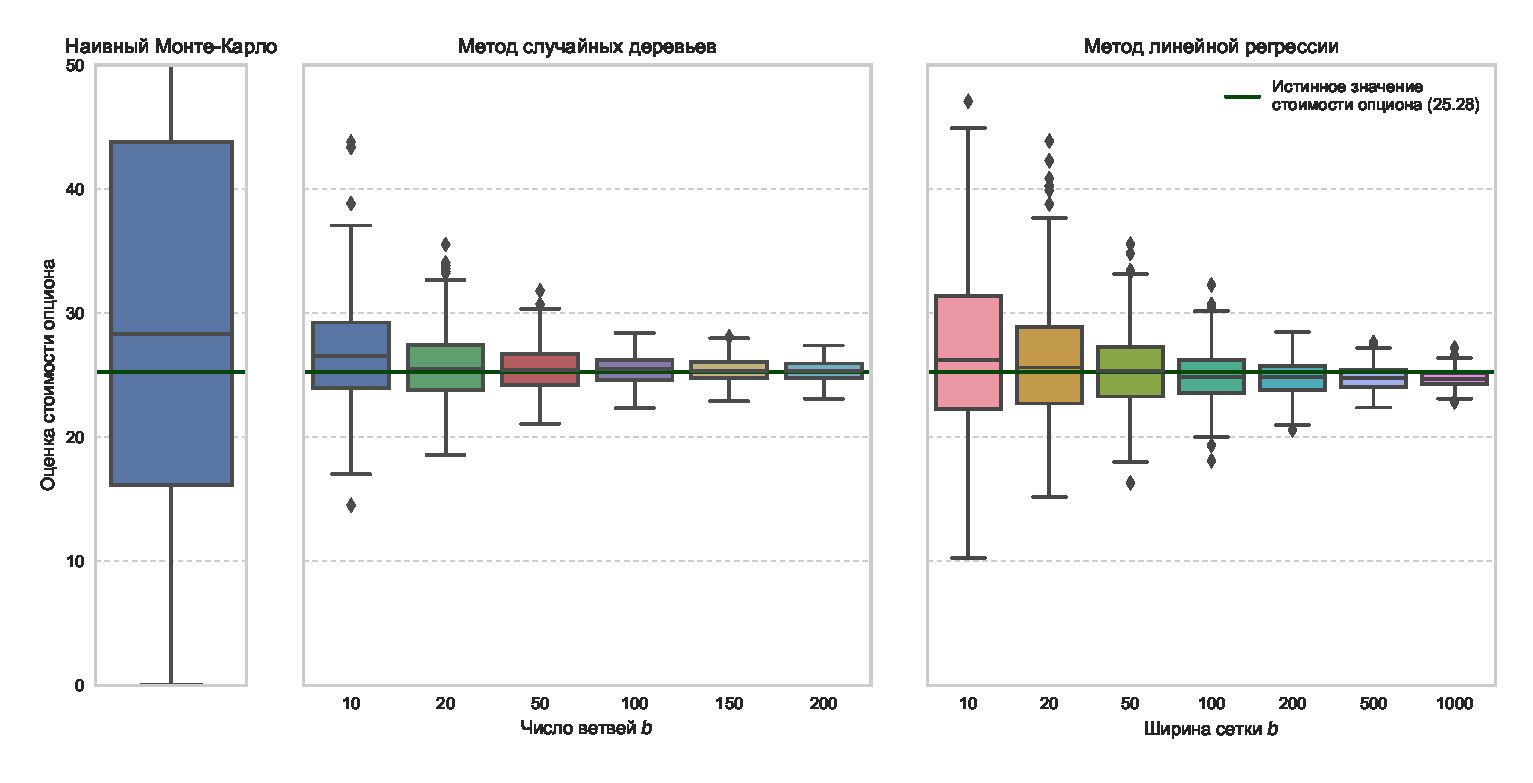
\includegraphics[width=\textwidth]{classical_methods.eps}
    \caption{Оценки стоимости опциона различными классическими методами}
    \footnotesize Оценки построены для примера \ref{example_3}. Из метода случайных деревьев взята оценка сверху. Вертикальная ось общая у всех трёх графиков.
    \label{fig:classical_methods}
\end{figure}

Здесь видно, что примерно одинаковый размер дисперсии (ориентироваться здесь имеет смысл на интерквартильный размах множества оценок, то есть высоту изображённого ящика) достигается в методе случайных деревьев при $b=100$ и в методе наименьших квадратов при $b=500$. Для случайного дерева для такого результата потребуется $\mathrm{dim} X_t \sum_{i=1}^{m-1 b^i} = 5 \cdot {1,010,100}$ обращений к генератору псевдослучайных чисел (обращения к генератору можно считать элементарной операцией, по количеству которых сравнивать время работы различных методов). В методе наименьших квадратов этот результат достигается за $\mathrm{dim} X_t \cdot (m-1)b = 5 \cdot 1500$ обращений, то есть оценку с той же дисперсией можно получить за гораздо меньшее время.

% section results:classical_approaches (end)

\section{Применение метода квази Монте-Карло к классическим методам} % (fold)
\label{sec:results:qmc_to_classical_methods}

В этом разделе обсуждаются результаты применения квази Монте-Карло к методам из предыдущей секции: методу случайных деревьев и методу наименьших квадратов. Были использованы две различные квазислучайные последовательности: квазислучайные числа Соболя \cite{NIEDERREITER198851} и квазислучайные числа Холтона \cite{Faure2009}.

Малые значения параметров алгоритмов используются специально для того, чтобы было возможным применить QMC и осуществить сравнение. В том числе по этой же причине сравнение приводится только для первых трёх примеров из списка выше: пример\,\ref{example_4} требует слишком большой размерности алгоритма для оценки. Несомненно, ограничения на размерность существующих последовательностей с низким дискрепансом серьёзно ограничивают область применения квазислучайных методов. Тем не менее, задачей работы было исследование самой возможности применения QMC для интегрирования сложных негладких функций (которой является стоимость Американского опциона), поэтому дискуссия о повышении размерности квазислучайной последовательности остаётся за рамками обсуждения.

Для каждой из последовательностей и каждого метода ниже приведено сравнение смещения и дисперсии (там, где её можно посчитать) оценок, полученных с использованием MC, QMC и RQMC. Подробное описание методики подсчёта дисперсии, стандартного отклонения и смещения приведено в секции \ref{ssub:qmc:randomization:variance_estimation}. Для каждой оценки было посчитано $N = 15,000$ реализаций, разделённых на $g = 600$ групп по $G = 25$ реализаций в каждой. 

\subsection{Последовательность Соболя} % (fold)
\label{sub:results:qmc_to_classical:sobol}

Квазислучайные числа Соболя показывают хорошие результаты интегрирования в умеренно высоких размерностях (см. \cite{sobol}). Примеры с использованием квазислучайных последовательностей Соболя различных размерностей посчитаны для размерностей, не превышающих 40. То есть, к примеру, если КРА (конструктивная размерность алгоритма) оценки по методу случайных деревьев превышает 40, то эта оценка не считается и не присутствует в таблицах результатов.

\subsubsection{Метод наименьших квадратов} % (fold)
\label{ssub:results:qmc_to_classical:sobol:lsm}

Результаты представлены на рис.\,\ref{fig:lsm_sobol} и в табл.\,\ref{tbl:lsm_sobol_ex1},\,\ref{tbl:lsm_sobol_ex2},\,\ref{tbl:lsm_sobol_ex3}.

\begin{figure}[p]
    \begin{center}
    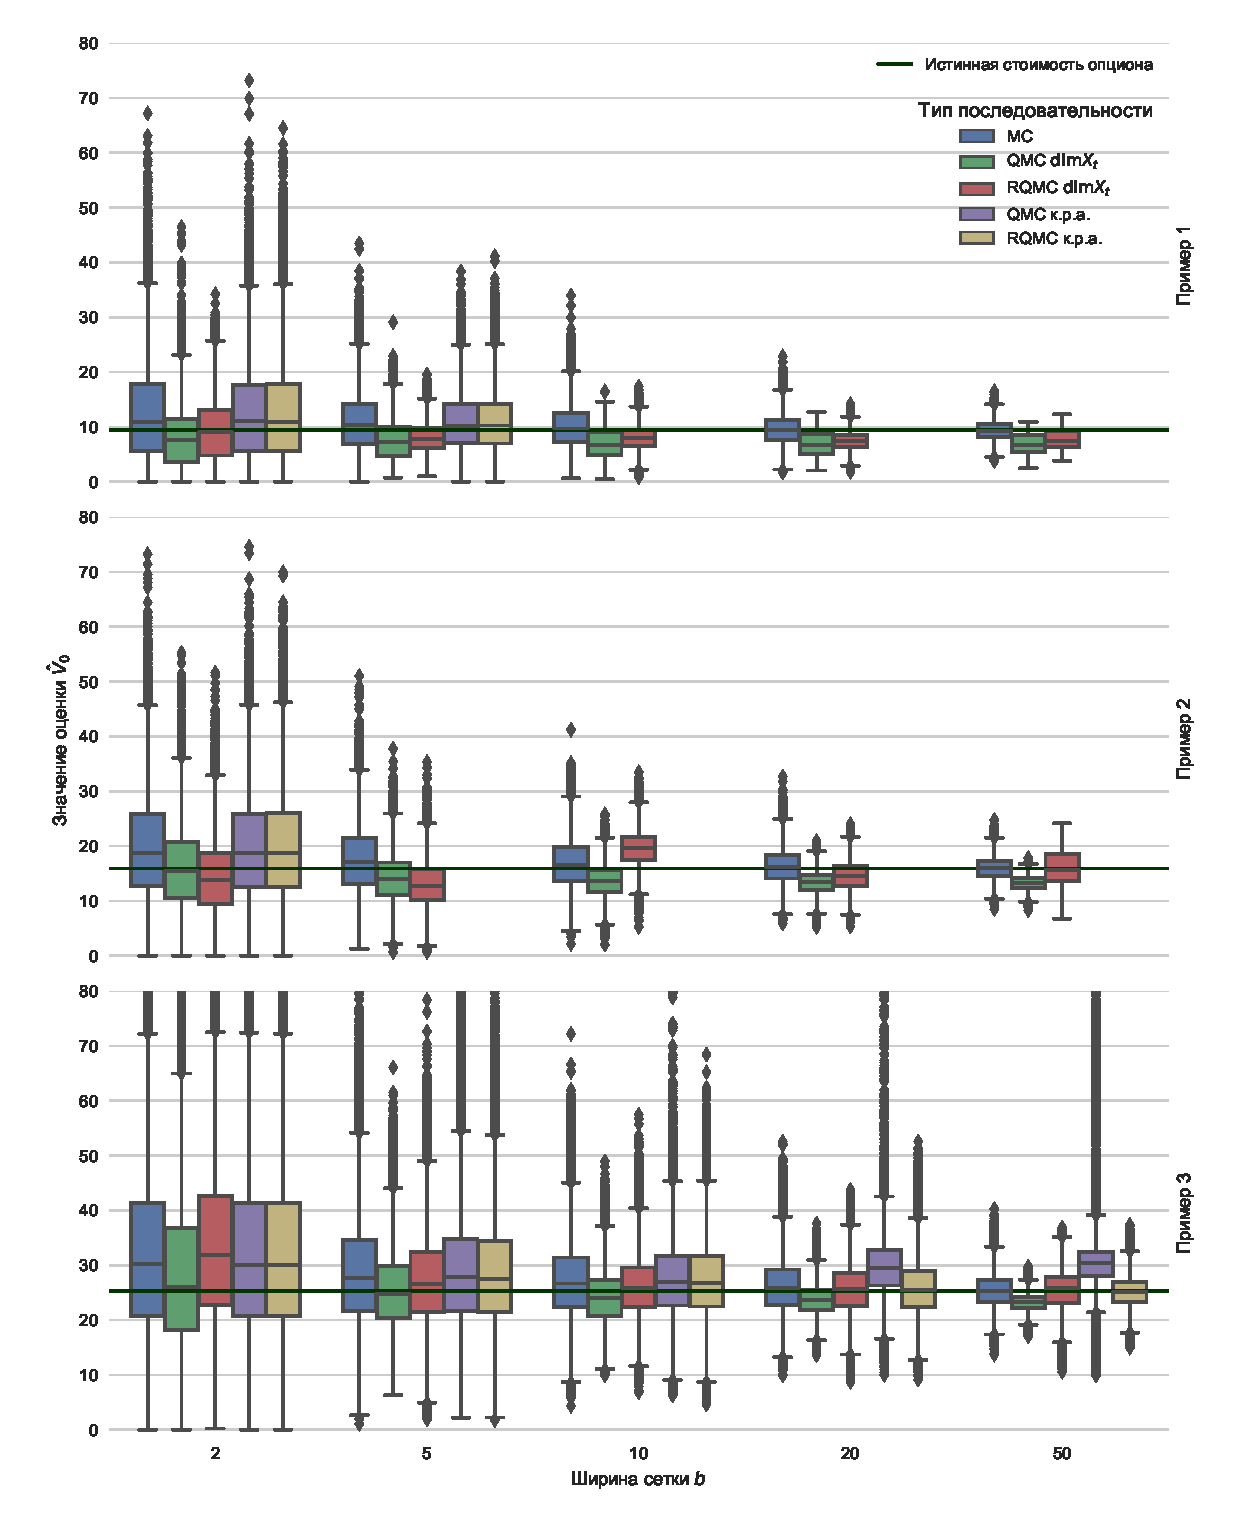
\includegraphics[width=0.9\textwidth]{lsm_sobol.eps}
    \end{center}
    \caption{Разброс оценок стоимости Американского опциона методом наименьших квадратов при использовании псевдослучайных последовательностей и квазислучайных последовательностей Соболя различных размерностей}
    \label{fig:lsm_sobol}

    \linespread{0.8}\footnotesize{На рисунке изображён именно разброс оценок, полученных при использовании различных отрезков квази- или псевдослучайной последовательности: подсчёт дисперсии и доверительных интервалов в случае QMC невозможен.}
\end{figure}

\begin{table}
    \renewcommand{\arraystretch}{0.6}
    \centering
    Оценки методом наименьших квадратов с псевдослучайной последовательностью (MC) и квазислучайной последовательностью Соболя (QMC)
    \caption{Пример 1}\label{tbl:lsm_sobol_ex1}
    \begin{tabular}{rrrrrrr}
        $b$&тип&$\mathrm{dim} X_t$&$\Vhat$&$\mathrm{sd}\Vhat$&$\mathrm{se}\Vhat$&$\mathrm{bias}\Vhat$\\[3pt]\hline\\[-8pt]
        2&MC&&12.562&1.856&3.700&3.201\\
        2&RQMC&2&9.516&1.112&1.123&0.155\\
        2&RQMC&12&12.535&1.139&3.372&3.174\\[3pt]
        5&MC&&10.992&1.045&1.937&1.631\\
        5&RQMC&2&7.938&0.606&1.546&-1.423\\
        5&RQMC&30&10.957&0.843&1.806&1.596\\[3pt]
        % 10&MC&&10.054&0.790&1.051&0.693\\
        % 10&RQMC&2&7.893&0.592&1.583&-1.468\\[3pt]
        % 20&MC&&9.562&0.501&0.540&0.201\\
        % 20&RQMC&2&7.403&0.697&2.078&-1.958\\[3pt]
        % 50&MC&&9.306&0.356&0.360&-0.055\\
        % 50&RQMC&2&7.673&1.480&2.245&-1.688\\[3pt]
    \end{tabular}

    \caption{Пример 2}\label{tbl:lsm_sobol_ex2}
    \begin{tabular}{rrrrrrr}
        $b$&тип&$\mathrm{dim} X_t$&$\Vhat$&$\mathrm{sd}\Vhat$&$\mathrm{se}\Vhat$&$\mathrm{bias}\Vhat$\\[3pt]\hline\\[-8pt]
        2&MC&&19.907&2.077&4.513&4.007\\
        2&RQMC&5&14.446&1.154&1.856&-1.454\\
        2&RQMC&30&19.851&1.528&4.236&3.951\\[3pt]
        5&MC&&17.557&1.270&2.088&1.657\\
        5&RQMC&5&13.058&1.205&3.087&-2.842\\[3pt]
        % 10&MC&&16.819&0.953&1.324&0.919\\
        % 10&RQMC&5&19.535&1.231&3.838&3.635\\[3pt]
        % 20&MC&&16.353&0.645&0.788&0.453\\
        % 20&RQMC&5&14.560&1.754&2.207&-1.340\\[3pt]
        % 50&MC&&15.983&0.435&0.443&0.083\\
        % 50&RQMC&5&15.958&2.682&2.682&0.058\\[3pt]
    \end{tabular}

    \caption{Пример 3}\label{tbl:lsm_sobol_ex3}
    \begin{tabular}{rrrrrrr}
        $b$&тип&$\mathrm{dim} X_t$&$\Vhat$&$\mathrm{sd}\Vhat$&$\mathrm{se}\Vhat$&$\mathrm{bias}\Vhat$\\[3pt]\hline\\[-8pt]
        2&MC&&32.438&3.421&7.934&7.158\\
        2&RQMC&30&32.285&7.987&10.623&7.005\\
        2&RQMC&5&35.431&1.825&10.314&10.151\\[3pt]
        5&MC&&28.570&1.990&3.845&3.290\\
        5&RQMC&5&25.258&2.010&2.010&-0.022\\[3pt]
        % 10&MC&&27.099&1.434&2.316&1.819\\
        % 10&RQMC&5&23.328&4.522&4.926&-1.952\\[3pt]
        % 20&MC&&26.110&0.941&1.255&0.830\\
        % 20&RQMC&5&26.001&0.943&1.187&0.721\\[3pt]
        % 50&MC&&25.418&0.605&0.621&0.138\\
        % 50&RQMC&5&24.545&2.455&2.563&-0.735\\[3pt]
    \end{tabular}

    \footnotesize{Расшифровку обозначений см.~в~\ref{eq:rqmc_variance_estimation}}
\end{table}

Результаты показывают, что использование квазислучайной последовательности Соболя размерности КРА снижает дисперсию оценки. Как и ожидалось, оценки с помощью квазислучайной последовательности размерности $\mathrm{dim} X$ не дают содержательных результатов: для некоторых случаев дисперсия меньше, чем в MC (пример 1, $b=2,5,10$; пример 2, $b=2$), для других --- меньше.

% subsubsection results:qmc_to_classical:sobol:lsm (end)

\subsubsection{Метод случайных деревьев} % (fold)
\label{ssub:results:qmc_to_classical:sobol:random_tree}

Результаты представлены на рис.\,\ref{fig:random_tree_sobol} и в табл.\,\ref{tbl:random_tree_sobol_ex1}.%,\,\ref{tbl:random_tree_sobol_ex2},\,\ref{tbl:random_tree_sobol_ex3}.

\begin{figure}[p]
    \begin{center}
    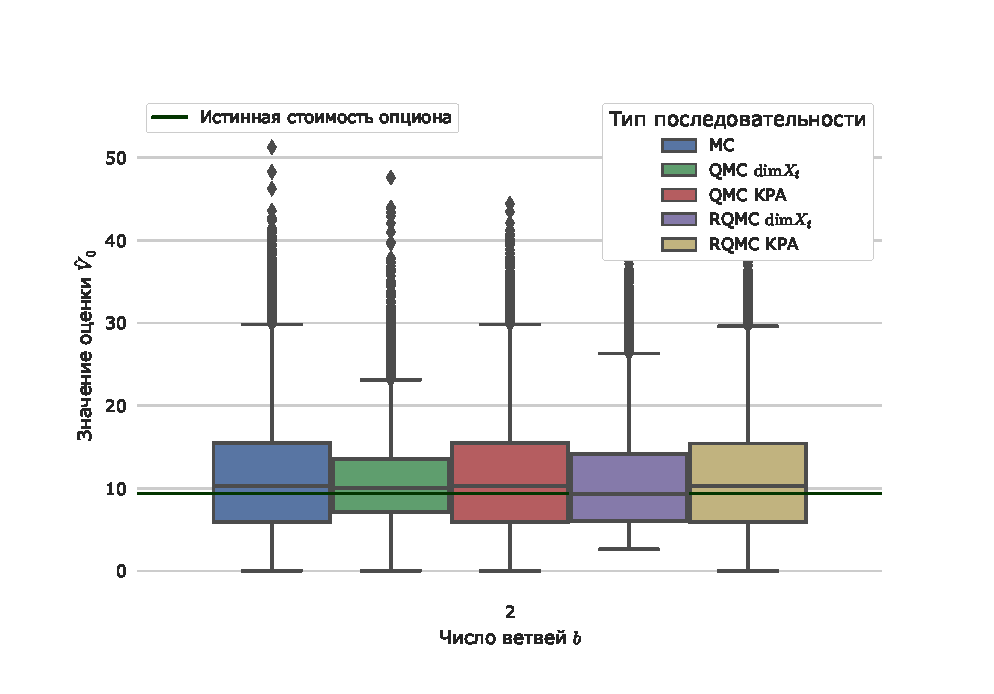
\includegraphics[width=0.9\textwidth]{random_tree_sobol.eps}\end{center}
    \caption{Разброс оценок стоимости Американского опциона методом случайных деревьев при использовании псевдослучайных последовательностей и квазислучайных последовательностей Соболя различных размерностей}
    \label{fig:random_tree_sobol}
    \linespread{0.8}\footnotesize{На рисунке изображён именно разброс оценок, полученных при использовании различных отрезков квази- или псевдослучайной последовательности: подсчёт дисперсии и доверительных интервалов в случае QMC невозможен.}
\end{figure}

\begin{table}
    \renewcommand{\arraystretch}{0.6}
    \centering
    Оценки методом случайных деревьев с псевдослучайной последовательностью (MC) и квазислучайной последовательностью Соболя (QMC)
    \caption{Пример 1}\label{tbl:random_tree_sobol_ex1}
    \begin{tabular}{rrrrrrr}
        $b$&тип&$\mathrm{dim} X_t$&$\Vhat$&$\mathrm{sd}\Vhat$&$\mathrm{se}\Vhat$&$\mathrm{bias}\Vhat$\\[3pt]\hline\\[-8pt]
        2&MC&&11.232&1.456&2.370&1.871\\
        2&RQMC&2&10.983&0.638&1.743&1.622\\
        2&RQMC&28&11.275&0.801&2.075&1.914\\[3pt]
        5&MC&&10.324&0.762&1.228&0.963\\
        5&RQMC&2&9.617&0.280&0.380&0.256\\[3pt]
  %       10&MC&&9.918&0.448&0.715&0.557\\
  %       10&RQMC&2&9.529&0.271&0.319&0.168\\[3pt]
  %       20&MC&&9.682&0.333&0.463&0.321\\
		% 20&RQMC&2&9.429&0.133&0.150&0.068\\[3pt]
    \end{tabular}

    % \caption{Пример 2}\label{tbl:random_tree_sobol_ex2}
    % \begin{tabular}{rrrrrrr}
    %     $b$&тип&$\mathrm{dim} X_t$&$\Vhat$&$\mathrm{sd}\Vhat$&$\mathrm{se}\Vhat$&$\mathrm{bias}\Vhat$\\[3pt]\hline\\[-8pt]
    %     2&MC&&17.934&1.570&2.570&2.034\\
    %     2&RQMC&5&19.065&2.004&3.746&3.165\\[3pt]
    %     5&MC&&16.990&0.807&1.356&1.090\\
    %     5&RQMC&5&17.414&3.428&3.748&1.514\\[3pt]
    %     10&MC&&16.499&0.536&0.803&0.599\\
    %     10&RQMC&5&18.016&3.273&3.897&2.116\\[3pt]
    % \end{tabular}

    % \caption{Пример 3}\label{tbl:random_tree_sobol_ex3}
    % \begin{tabular}{rrrrrrr}
    %     $b$&тип&$\mathrm{dim} X_t$&$\Vhat$&$\mathrm{sd}\Vhat$&$\mathrm{se}\Vhat$&$\mathrm{bias}\Vhat$\\[3pt]\hline\\[-8pt]
    %     2&MC&&29.502&2.432&4.873&4.222\\
    %     2&RQMC&5&26.231&2.573&2.743&0.951\\[3pt]
    %     5&MC&&27.207&1.228&2.285&1.927\\
    %     5&RQMC&5&27.666&2.017&3.124&2.386\\[3pt]
    %     10&MC&&26.353&0.811&1.346&1.073\\
    %     10&RQMC&5&26.673&1.720&2.213&1.393\\[3pt]
    % \end{tabular}

    \footnotesize{Расшифровку обозначений см.~в~\ref{eq:rqmc_variance_estimation}}
\end{table}

При использовании метода случайных деревьев только в одном случае КРА достаточно мала, чтобы строить оценку с использованием квазислучайной последовательности размерности, равной КРА. При этом остаётся неясным, насколько точными являются полученные оценки $\mathrm{sd}\Vhat$ и $\mathrm{se}\Vhat$ (возможно, если взять размер выборки $N$ чуть больше или чуть меньше, то отношение между $\mathrm{sd}\Vhat$ для MC и RQMC существенно изменится?). Одним из способов оценить поведение оценок является рис.\,\ref{fig:random_tree_sobol_variance}, на котором обсуждаемые оценки стандартного и среднеквадратичного отклонения изображены как функции от размера выборки. Он показывает, что оценки отклонений вполне статичны и преимущество RQMC в этом случае не является случайным эффектом малой выборки.

\begin{figure}[h!bt]
    \begin{center}
    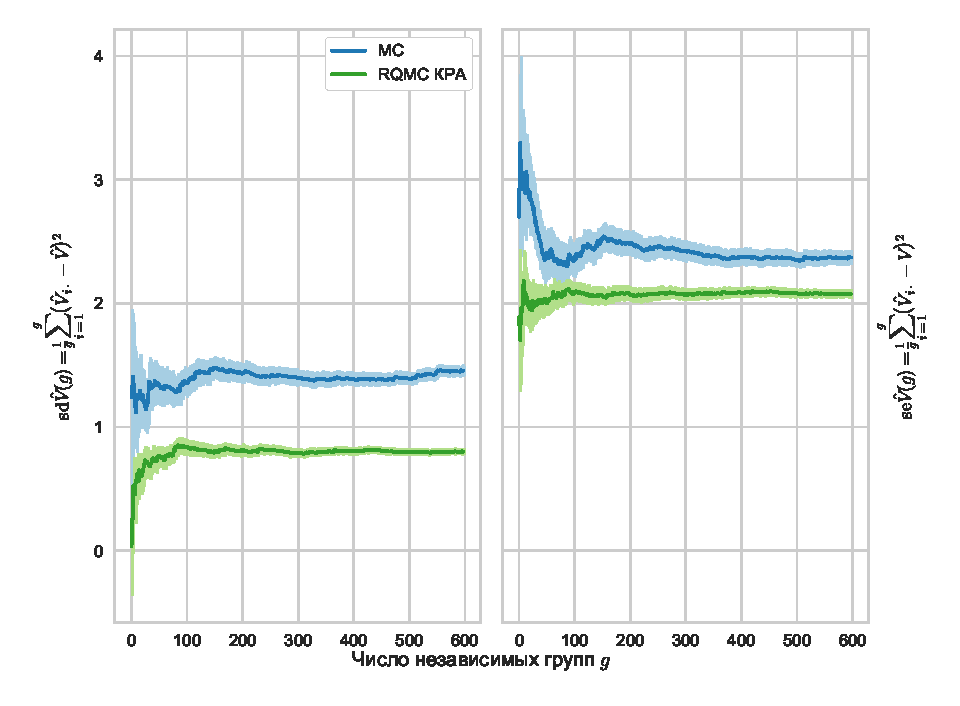
\includegraphics[width=0.9\textwidth]{random_tree_sobol_variance.eps}\end{center}
    \caption{Оценки $\mathrm{sd}\Vhat$ и $\mathrm{se}\Vhat$ в зависимости от размера выборки}
    \label{fig:random_tree_sobol_variance}
    \linespread{0.7}\footnotesize{
        Оценки стандартного и среднеквадратичного отклонения оценки стоимости Американского опциона из примера \ref{example_1} при использовании метода случайных деревьев с MC и RQMC Соболя размерности КРА. Количество коррелированных оценок в группе постоянно и равно $G=25$, при росте $g$ увеличивается размер выборки $N=g\cdot G$. Значения крайних правых точек графика указаны в табл.\,\ref{tbl:random_tree_sobol_ex1}. Значение оценки на выборке из первых $g$ групп указано более тёмной линией, более бледным обозначено стандартное отклонение этой оценки, посчитанное с помощью бутстрепа.}
\end{figure}

% subsubsection results:qmc_to_classical:sobol:random_tree (end)

% subsection results:qmc_to_classical:sobol (end)

\subsection{Последовательность Холтона} % (fold)
\label{sub:results:qmc_to_classical:halton}

Примеры с использованием квазислучайных последовательностей Холтона различных размерностей посчитаны для размерностей $< 40$. Стоит отметить, что в силу своей конструкции последовательности Холтона обычно не показывают хороших результатов при численном интегрировании в умеренно высоких размерностях (см., например, \cite{Faure2009}).

\subsubsection{Метод наименьших квадратов} % (fold)
\label{ssub:results:qmc_to_classical:halton:lsm}

Результаты представлены на рис.\,\ref{fig:lsm_halton} и в табл.\,\ref{tbl:lsm_halton_ex1},\,\ref{tbl:lsm_halton_ex2},\,\ref{tbl:lsm_halton_ex3}.

\begin{figure}[p]
    \begin{center}
    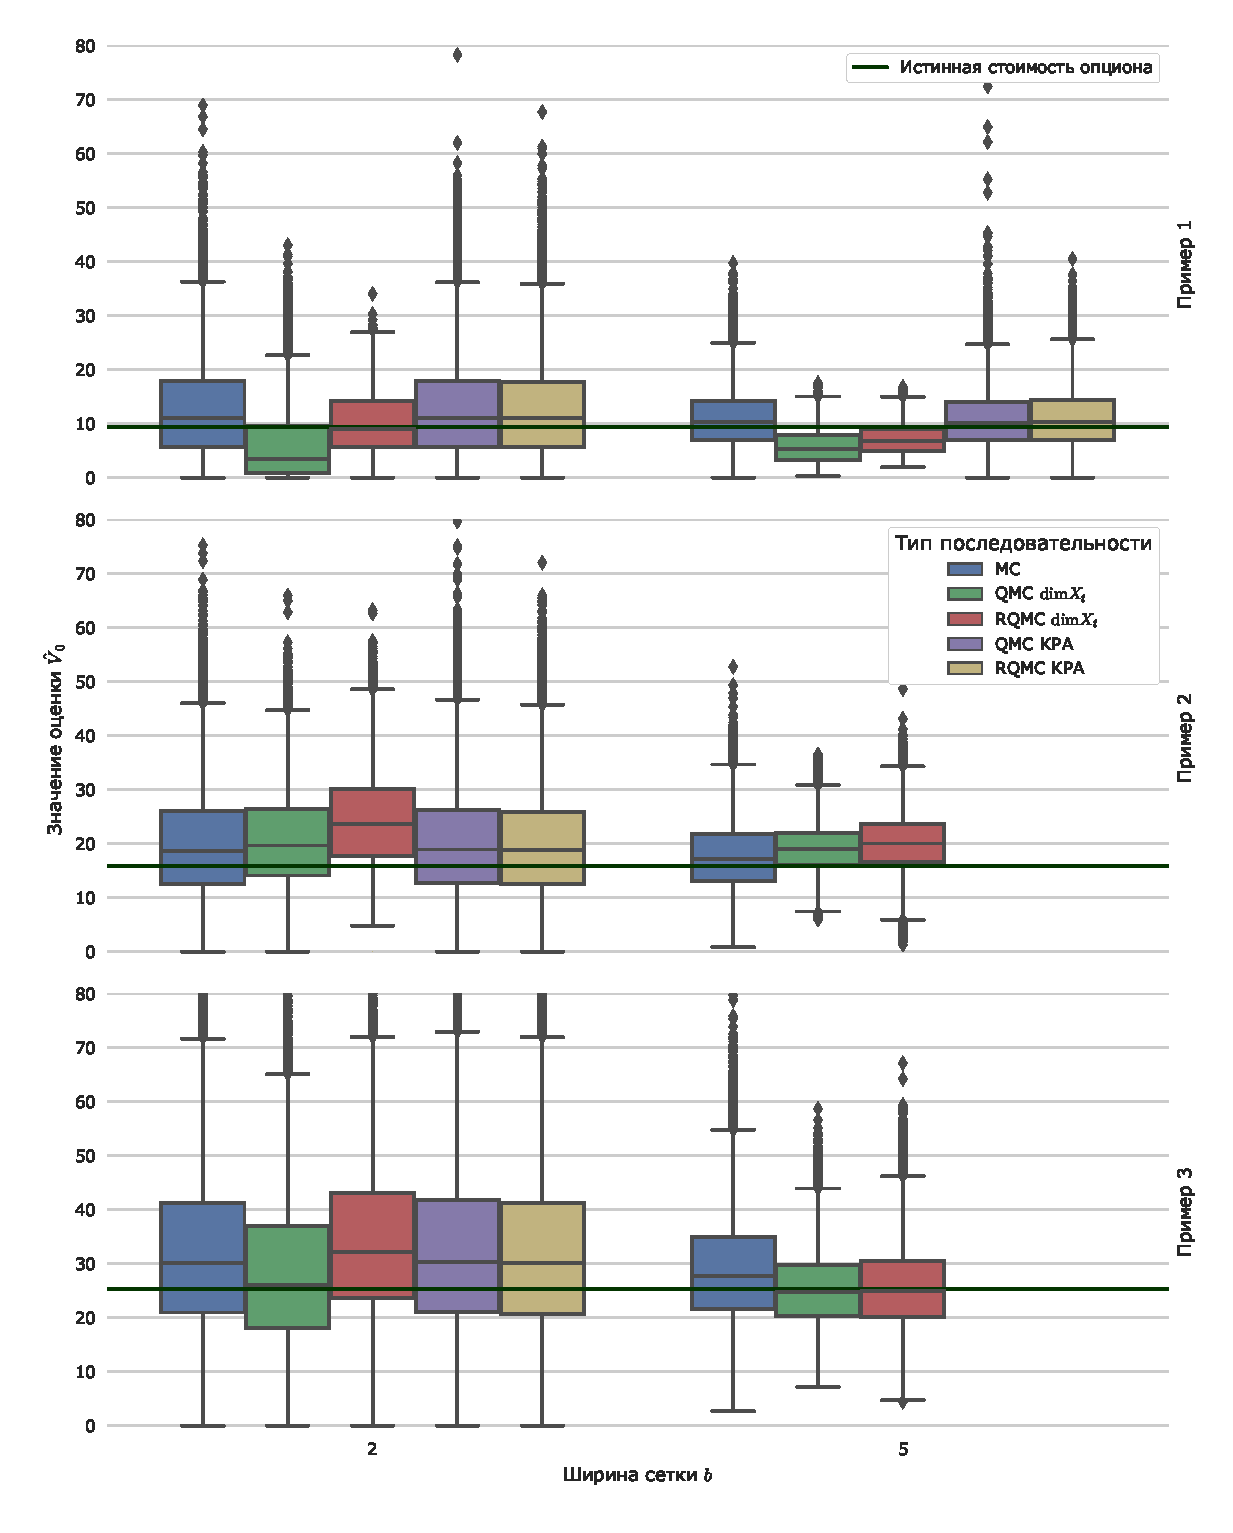
\includegraphics[width=0.9\textwidth]{lsm_halton.eps}\end{center}
    \caption{Разброс оценок стоимости Американского опциона методом наименьших квадратов при использовании псевдослучайных последовательностей и квазислучайных последовательностей Холтона различных размерностей}
    \label{fig:lsm_halton}
    \linespread{0.8}\footnotesize{На рисунке изображён именно разброс оценок, полученных при использовании различных отрезков квази- или псевдослучайной последовательности: подсчёт дисперсии и доверительных интервалов в случае QMC невозможен.}
\end{figure}

\begin{table}
    \renewcommand{\arraystretch}{0.6}
    \centering
    Оценки методом наименьших квадратов с псевдослучайной последовательностью и квазислучайной последовательностью Холтона
    \caption{Пример 1}\label{tbl:lsm_halton_ex1}
    \begin{tabular}{rrrrrrr}
        $b$&тип&$\mathrm{dim} X_t$&$\Vhat$&$\mathrm{sd}\Vhat$&$\mathrm{se}\Vhat$&$\mathrm{bias}\Vhat$\\[3pt]\hline\\[-8pt]
        2&MC&&12.535&1.818&3.658&3.174\\
        2&RQMC&12&12.540&2.339&3.947&3.179\\
        2&RQMC&2&6.119&0.543&3.287&-3.242\\[3pt]
        5&MC&&10.979&1.094&1.953&1.618\\
        5&RQMC&30&10.967&2.810&3.237&1.606\\
        5&RQMC&2&7.349&0.208&2.023&-2.012\\[3pt]
        10&MC&&10.120&0.736&1.058&0.759\\
        10&RQMC&2&11.696&0.117&2.338&2.335\\[3pt]
        % 20&MC&&9.639&0.549&0.615&0.278\\
        % 20&RQMC&2&11.867&0.064&2.507&2.506\\[3pt]
        % 50&MC&&9.292&0.348&0.355&-0.069\\
        % 50&RQMC&2&7.701&3.284&3.680&-1.660\\[3pt]
    \end{tabular}

    \caption{Пример 2}\label{tbl:lsm_halton_ex2}
    \begin{tabular}{rrrrrrr}
        $b$&тип&$\mathrm{dim} X_t$&$\Vhat$&$\mathrm{sd}\Vhat$&$\mathrm{se}\Vhat$&$\mathrm{bias}\Vhat$\\[3pt]\hline\\[-8pt]
        2&MC&&19.753&1.956&4.321&3.853\\
        2&RQMC&30&19.860&5.361&6.665&3.960\\
        2&RQMC&5&15.481&0.713&0.827&-0.419\\[3pt]
        5&MC&&17.478&1.243&2.009&1.578\\
        5&RQMC&5&19.220&0.622&3.377&3.320\\[3pt]
        % 10&MC&&16.822&0.903&1.291&0.922\\
        % 10&RQMC&5&15.008&3.358&3.474&-0.892\\[3pt]
        % 20&MC&&16.272&0.653&0.751&0.372\\
        % 20&RQMC&5&15.612&3.711&3.722&-0.288\\[3pt]
        % 50&MC&&16.011&0.429&0.443&0.111\\
        % 50&RQMC&5&16.647&3.263&3.348&0.747\\[3pt]
    \end{tabular}

    \caption{Пример 3}\label{tbl:lsm_halton_ex3}
    \begin{tabular}{rrrrrrr}
        $b$&тип&$\mathrm{dim} X_t$&$\Vhat$&$\mathrm{sd}\Vhat$&$\mathrm{se}\Vhat$&$\mathrm{bias}\Vhat$\\[3pt]\hline\\[-8pt]
        2&MC&&32.438&3.421&7.934&7.158\\
        2&RQMC&30&32.285&7.987&10.623&7.005\\
        2&RQMC&5&35.431&1.825&10.314&10.151\\[3pt]
        5&MC&&28.570&1.990&3.845&3.290\\
        5&RQMC&5&25.258&2.010&2.010&-0.022\\[3pt]
        % 10&MC&&27.099&1.434&2.316&1.819\\
        % 10&RQMC&5&23.328&4.522&4.926&-1.952\\[3pt]
        % 20&MC&&26.110&0.941&1.255&0.830\\
        % 20&RQMC&5&26.001&0.943&1.187&0.721\\[3pt]
        % 50&MC&&25.418&0.605&0.621&0.138\\
        % 50&RQMC&5&24.545&2.455&2.563&-0.735\\[3pt]
    \end{tabular}

    \footnotesize{Расшифровку обозначений см.~в~\ref{eq:rqmc_variance_estimation}}
\end{table}

Из таблиц \ref{tbl:lsm_halton_ex1},\,\ref{tbl:lsm_halton_ex2} видно, что на тех же примерах, где использование последовательность Соболя размерности, равной КРА, давало выигрыш в дисперсии, использование последовательности Холтона существенно увеличивает дисперсию. %Можно предположить, что эта разница объясняется тем, что в выборке слишком мало примеров. Но рис.\ref показывает, что во всех случаях оценки достаточно стабильны.

% subsubsection results:qmc_to_classical:halton:lsm (end)

\subsubsection{Метод случайных деревьев} % (fold)
\label{ssub:results:qmc_to_classical:halton:random_tree}

Результаты представлены на рис.\,\ref{fig:random_tree_halton} и в табл.\,\ref{tbl:random_tree_halton_ex1}.%,\,\ref{tbl:random_tree_halton_ex2},\,\ref{tbl:random_tree_halton_ex3}.

\begin{figure}[p]
    \begin{center}
    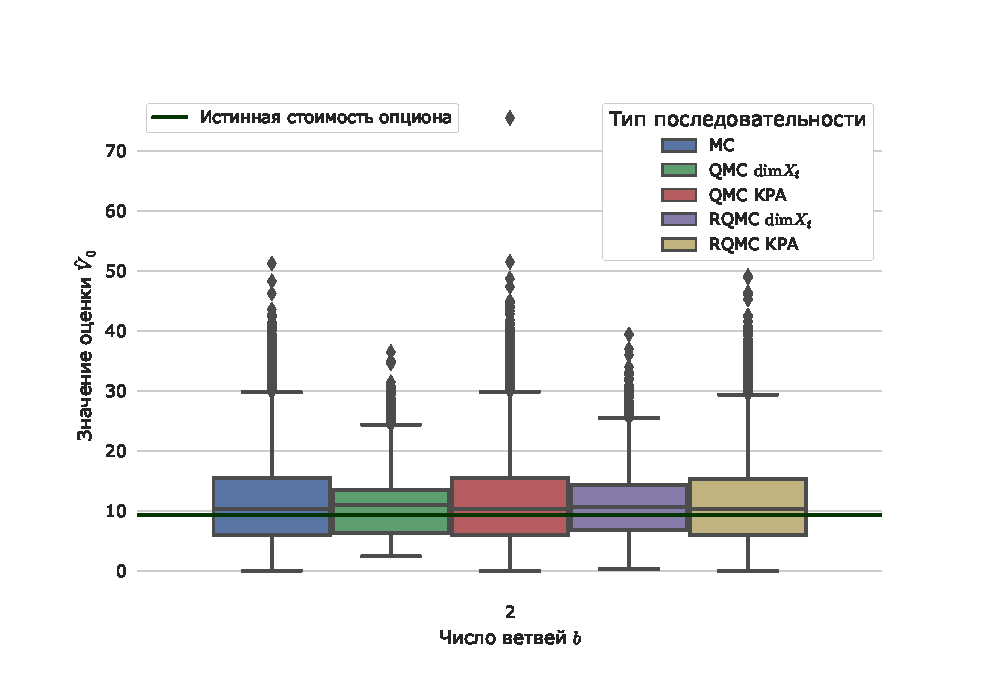
\includegraphics[width=0.9\textwidth]{random_tree_halton.eps}\end{center}
    \caption{Разброс оценок стоимости Американского опциона методом случайных деревьев при использовании псевдослучайных последовательностей (MC) и квазислучайных последовательностей Холтона (QMC) различных размерностей}
    \label{fig:random_tree_halton}
    \linespread{0.8}\footnotesize{На рисунке изображён именно разброс оценок, полученных при использовании различных отрезков квази- или псевдослучайной последовательности: подсчёт дисперсии и доверительных интервалов в случае QMC невозможен.}
\end{figure}

\begin{table}
    \renewcommand{\arraystretch}{0.6}
    \centering
    Оценки методом случайных деревьев с псевдослучайной последовательностью (MC) и квазислучайной последовательностью Холтона (QMC)
    \caption{Пример 1}\label{tbl:random_tree_halton_ex1}
    \begin{tabular}{rrrrrrr}
        $b$&тип&$d$&$\Vhat$&$\mathrm{sd}\Vhat$&$\mathrm{se}\Vhat$&$\mathrm{bias}\Vhat$\\[3pt]\hline\\[-8pt]
        2&MC&&11.232&1.456&2.370&1.871\\
        2&RQMC&2&11.014&0.429&1.708&1.653\\
        2&RQMC&28&11.273&1.969&2.745&1.912\\[3pt]
        5&MC&&10.324&0.762&1.228&0.963\\
        5&RQMC&2&9.879&0.217&0.562&0.518\\[3pt]
  %       10&MC&&9.918&0.448&0.715&0.557\\
  %       10&RQMC&2&9.559&0.465&0.505&0.198\\[3pt]
  %       20&MC&&9.682&0.333&0.463&0.321\\
  %       20&RQMC&2&9.423&0.110&0.126&0.062\\[3pt]
  %       50&MC&&9.490&0.190&0.230&0.129\\
		% 50&RQMC&2&9.376&0.041&0.044&0.015\\[3pt]
    \end{tabular}

    % \centering
    % \caption{Пример 2}\label{tbl:random_tree_halton_ex2}
    % \begin{tabular}{rrrrrrr}
    %     $b$&тип&$d$&$\Vhat$&$\mathrm{sd}\Vhat$&$\mathrm{se}\Vhat$&$\mathrm{bias}\Vhat$\\[3pt]\hline\\[-8pt]
    %     2&MC&&17.934&1.570&2.570&2.034\\
    %     2&RQMC&5&20.616&1.608&4.982&4.716\\[3pt]
    %     5&MC&&16.990&0.807&1.356&1.090\\
    %     5&RQMC&5&16.666&2.346&2.467&0.766\\[3pt]
    %     10&MC&&16.499&0.536&0.803&0.599\\
    %     10&RQMC&5&16.919&2.904&3.078&1.019\\[3pt]
    %     20&MC&&16.193&0.351&0.458&0.293\\
    %     20&RQMC&5&16.510&2.216&2.299&0.610\\[3pt]
    % \end{tabular}

    % \centering
    % \caption{Пример 3}\label{tbl:random_tree_halton_ex3}
    % \begin{tabular}{rrrrrrr}
    %     $b$&тип&$d$&$\Vhat$&$\mathrm{sd}\Vhat$&$\mathrm{se}\Vhat$&$\mathrm{bias}\Vhat$\\[3pt]\hline\\[-8pt]
    %     2&MC&&29.502&2.432&4.873&4.222\\
    %     2&RQMC&5&28.972&2.018&4.208&3.692\\[3pt]
    %     5&MC&&27.207&1.228&2.285&1.927\\
    %     5&RQMC&5&27.505&1.984&2.981&2.225\\[3pt]
    %     10&MC&&26.353&0.811&1.346&1.073\\
    %     10&RQMC&5&26.786&1.730&2.293&1.506\\[3pt]
    %     20&MC&&25.826&0.533&0.763&0.546\\
    %     20&RQMC&5&26.281&1.407&1.727&1.001\\[3pt]
    % \end{tabular}

    \footnotesize{Расшифровку обозначений см.~в~\ref{eq:rqmc_variance_estimation}}
\end{table}

Здесь, как и в случае с последовательностью Соболя (см. секцию\,\ref{ssub:results:qmc_to_classical:sobol:random_tree}), для КРА есть только одно наблюдение, поэтому стоит посмотреть на поведение отклонений в зависимости от размера выборки. Оно изображено на рис.\,\ref{fig:random_tree_halton_variance}. Судя по представленному на графике поведению, оценка стандартного отклонения для 600 наблюдений достаточно устойчива, и оснований считать, что QMC размерности КРА превосходит MC, нет.

% Про использование размерности, равной размерности актива, как и в случае с последовательностью Соболя, никаких выводов сделать нельзя: на примере \ref{example_1} (табл.\,\ref{tbl:random_tree_halton_ex1}) рандомизированный квази Монте-Карло демонстрирует стандартное отклонение намного меньшее стандартного отклонения классического Монте-Карло, тогда как в примерах \ref{example_2} и \ref{example_3} (табл.\,\ref{tbl:random_tree_halton_ex2} и \ref{tbl:random_tree_halton_ex3}) результаты гораздо хуже стандартного Монте-Карло. Также присутствует дополнительное смещение оценки.

\begin{figure}[h]
    \begin{center}
    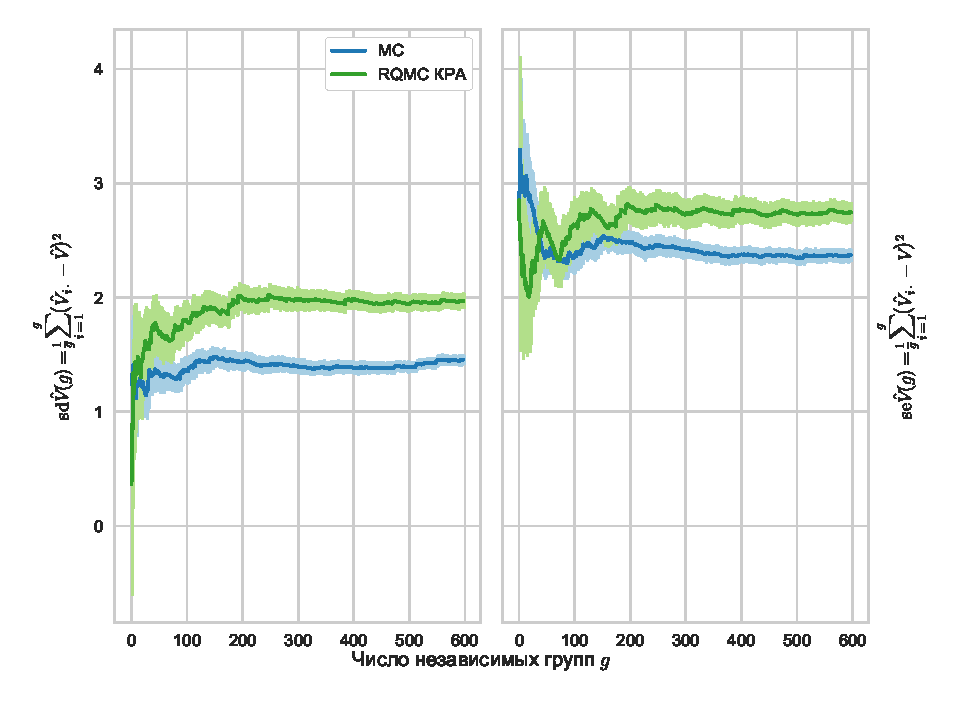
\includegraphics[width=0.9\textwidth]{random_tree_halton_variance.eps}\end{center}
    \caption{Оценки $\mathrm{sd}\Vhat$ и $\mathrm{se}\Vhat$ в зависимости от размера выборки}
    \label{fig:random_tree_halton_variance}
    \linespread{0.7}\footnotesize{
        Оценки стандартного и среднеквадратичного отклонения оценки стоимости Американского опциона из примера \ref{example_1} при использовании метода случайных деревьев с MC и c RQMC Холтона размерности, равной конструктивной размерности алгоритма. Количество коррелированных оценок в группе постоянно и равно $G=25$, при росте $g$ увеличивается размер выборки $N=g\cdot G$. Значения крайних правых точек графика указаны в табл.\,\ref{tbl:random_tree_sobol_ex1}. Значение оценки на выборке из первых $g$ групп указано более тёмной линией, более бледным обозначено стандартное отклонение этой оценки, посчитанное с помощью бутстрепа.}
\end{figure}

% subsubsection results:qmc_to_classical:halton:random_tree (end)

% subsection results:qmc_to_classical:halton (end)

Представленные в этом разделе результаты подтверждают, что последовательность Холтона плохо справляется с интегрированием в пространствах умеренно высокой размерности. Напротив, последовательность Соболя демонстрирует гораздо более хорошие результаты, чем классический Монте-Карло, даже в случае сложной негладкой функции.

% section results:qmc_to_classical_methods (end)

\section{Оценки по сглаженным случайным деревьям} % (fold)
\label{sec:results:pruned_trees}

Для сравнения алгоритмов требуется пример с известным ответом: Американский опцион с известными параметрами, для которого известна стоимость при условии возможности исполнения опциона в любой момент времени (т.е. при $m \to \infty$). Поэтому сравнение проводится для примера \ref{example_4}.

Оценка по сглаженным деревьям сравнивается с оценкой по методу наименьших квадратов. Параметры оценки по сглаженным деревьям ($b, h, n$) выбраны таким образом, чтобы доставлять наименьшую дисперсию при фиксированном $m$ и ограниченном сверху $n$. Параметр $b$ для метода наименьших квадратов выбирался таким образом, чтобы конструктивная размерность оценок совпадала. Сравнение дисперсий представлено на рис.\,\ref{fig:lsm_vs_pruned_variance}, и, согласно этим данным, дисперсия в методе сглаженных деревьев ниже.

\begin{figure}[h]
    \begin{center}
    \includegraphics[width=0.9\textwidth]{LSM_vs_pruned_variance.eps}\end{center}
    \caption{Дисперсия оценок по методу наименьших квадратов и методу сглаженных случайных деревьев}
    \label{fig:lsm_vs_pruned_variance}
\end{figure}

% section results:pruned_trees (end)

\section{Применение метода квази Монте-Карло к сглаженным случайным деревьям} % (fold)
\label{sec:results:qmc_to_pruned_trees}

Существует два наиболее очевидных варианта применения квази Монте-Карло к исследуемому методу:

\begin{enumerate}
	\item Использование QMC для генерирования более регулярной сетки на шаге выбора точек роста для новых деревьев: размерность QMC равна размерности базового актива, для генерации деревьев используется генератор псевдослучайных чисел (ГПСЧ).
	\item Использование QMC для генерации деревьев: размерность QMC равна $\mathrm{dim} X_t \cdot \sum_{i=1}^h b^i$, для выбора сетки используется ГПСЧ или другая QMC-последовательность (уже другой размерности).
\end{enumerate}

В таблицах далее эти варианты обозначаются суффиксами <<grid>> и <<tree>> соответственно. Сравнение оценок с использованием QMC с оценками с использованием MC приведено на рис.\,\ref{fig:pruned_tree_sobol} и в табл.\,\ref{tbl:pruned_tree_sobol}. Использовалась квазислучайная последовательность Соболя. Как видно из рисунка, использование QMC для генерации деревьев меньшую ошибку относительно истинного значения стоимости опциона. Это можно объяснить тем, что использование QMC для генерации сетки вершин обеспечивает более равномерную решётку, порождая более точные оценки линейной регрессии $\Vhat^{\mathrm{regr.}}_{p_l}$ и компенсируя тем самым один из источников смещения.

\begin{figure}[h]
    \begin{center}
    \includegraphics[width=0.9\textwidth]{pruned_tree_sobol.eps}\end{center}
    \caption{Разброс оценок стоимости Американского опциона методом сглаженных случайных деревьев при использовании псевдослучайных последовательностей (MC) и квазислучайных последовательностей Соболя (QMC) в различных частях алгоритма}
    \label{fig:pruned_tree_sobol}
    \linespread{0.8}\footnotesize{Вычисления представлены для примера \ref{example_4}. На рисунке изображён именно разброс оценок, полученных при использовании различных отрезков квази- или псевдослучайной последовательности: подсчёт дисперсии и доверительных интервалов в случае QMC невозможен.}
\end{figure}

Сведения из табл.\,\ref{tbl:pruned_tree_sobol} также демонстрируют, что использование рандомизированных квазислучайных методов не даёт большого выигрыша в дисперсии для оценки по сглаженным деревьям (по крайней мере, на исследуемом примере). При этом использование квазислучайных методов позволяет добиться разброса в значениях оценки по различным частям квазислучайной последовательности меньшего, чем в методе Монте-Карло (не указано в таблице).

\begin{table}
    \renewcommand{\arraystretch}{0.6}
    \centering
    \caption{Оценки методом сглаженных случайных деревьев при использовании псевдослучайных последовательностей (MC) и квазислучайных последовательностей Соболя (QMC) в различных частях алгоритма}\label{tbl:pruned_tree_sobol}
    \begin{tabular}{rrrrrrrrr}
    $b$&$h$&$m$&$n$&тип&$\Vhat$&$\mathrm{sd}\Vhat$&$\mathrm{se}\Vhat$&$\mathrm{bias}\Vhat$\\[3pt]\hline\\[-8pt]
    4&3&22&100&MC&12.952&0.371&3.336&3.315\\
    4&3&22&100&QMC grid&11.669&-&-&2.032\\
    4&3&22&100&QMC tree&2.373&-&-&-7.264\\
    4&3&22&100&RQMC grid&13.006&0.934&3.496&3.369\\
    4&3&22&100&RQMC tree&13.202&4.744&5.935&3.565\\[3pt]
    14&2&22&100&MC&13.321&0.224&3.691&3.684\\
    14&2&22&100&QMC grid&11.709&-&-&2.072\\
    14&2&22&100&QMC tree&2.532&-&-&-7.105\\
    14&2&22&100&RQMC grid&13.383&1.025&3.884&3.746\\
    14&2&22&100&RQMC tree&13.540&4.642&6.065&3.903\\[3pt]
    14&2&22&200&MC&13.379&0.208&3.748&3.742\\
    14&2&22&200&QMC grid&11.632&-&-&1.995\\
    14&2&22&200&QMC tree&2.458&-&-&-7.179\\
    14&2&22&200&RQMC grid&13.426&0.893&3.893&3.789\\
    14&2&22&200&RQMC tree&14.784&5.571&7.584&5.147\\[3pt]
    \end{tabular}
\end{table}
% section results:qmc_to_pruned_trees (end)
% chapter numerical_results (end)
%!TEX root = thesis.tex
\conclusion

В работе проведено исследование вопроса применимости метода квази Монте-Карло к задаче оценивания Американского опциона. Из приведённых результатов следует, что метод в целом применим к задаче. Разрешён вопрос о выборе размерности квазислучайной последовательности: в общем случае размерность, равная конструктивной размерности алгоритма, показывает наилучшие результаты. Подтверждены ранее известные сведения о неудовлетворительных результатах применения квазислучайных чисел Холтона в задачах численного интегрирования умеренно высокой размерности и продемонстрированы результаты для квазислучайных чисел Соболя, показывающие, что эта последовательность может быть успешно применена.

Также предложен новый алгоритм оценки стоимости Американских опционов\textcolor{gray}{, проведены численные сравнения алгоритма с существующими и доказана состоятельность оценок, получаемых с помощью предложенного алгоритма}.

% глоссарий: \E -- матожидание

% \intro
% В работе рассмотрены основные подходы к оценке стоимости Американских опционов и приведено их сравнение между собой (как теоретическое, так и на численных примерах). Основной целью работы было исследование вопроса о применении метода квази Монте-Карло к задаче оценки стоимости Американского опциона.

% В главе \ref{cha:option_price_estimation_problem} описана задача оценки Американских опционов (в секции \ref{sec:option_price}) и приведены основные методы её решения (случайные деревья, стохастические сетки и линейная регрессия, раздел \ref{sec:estimators}). 
% % Глава \ref{cha:variance_reduction} содержит описание методов снижения дисперсии оценок, в частности, применение квази Монте-Карло. 
% В главе \ref{cha:quasi_monte_carlo} более подробно разобрана теория квази Монте-Карло и приведены обоснования для выбора размерности квазислучайной последовательности. В большинстве секций теоретические сведения подкреплены демонстрацией вычислений на конкретных примерах.

% \chapter{Задача оценки стоимости Американского опциона} % (fold)
% \label{cha:option_price_estimation_problem}

% Опцион --- это широко распространённый вторичный (производный) финансовый инструмент. Опцион является контрактом между продавцом опциона и покупателем опциона о том, что покупатель имеет право, но не обязательство, купить (в случае опциона на покупку, call option) или продать (в случае опциона на продажу, put option) указанный в контракте базовый актив по заранее оговорённой цене в определённый контрактом момент в будущем или на протяжении определённого отрезка времени. Продавца опциона контракт обязует совершить ответную продажу (для опциона на покупку) или покупку (для опциона на продажу) в случае, если покупатель пожелает исполнить своё право. Реализация такой сделки называется \emph{исполнением опциона}.

% Различают опционы европейского и американского типа. Опцион европейского типа выписывается на фиксированный момент времени в будущем, опцион американского типа --- на отрезок времени. Промежуточный вариант, когда опцион может быть исполнен только в определённые даты (например, в конце каждого квартала в течение года), часто называют Бермудским опционом.

% Исполнение опциона может быть выгодно его владельцу (когда цена базового актива в контракте ниже текущей рыночной в случае опциона на покупку, когда цена базового актива выше текущей рыночной в случае опциона на продаже), поэтому опционный контракт сам по себе тоже имеет стоимость. Ищется стоимость опциона в модели эффективного рынка, то есть такая цена $V$, при которой ни продавец, ни покупатель опциона в среднем не получают прибыли.

% \section{Стоимость Американского опциона как случайная величина} % (fold)
% \label{sec:option_price}

% В случае опциона европейского типа существует решение в замкнутой форме (модель Блэка-Шоулса \cite{Black1973} и её усовершенствования). Оценка Американского опциона является более сложной задачей.

% Опцион определяется 
% \begin{itemize}[noitemsep,topsep=0pt]
% \item своим временем жизни $[0;T]$, 
% \item базовым активом $X$ (под $X(t)$ будем подразумевать состояние актива в момент времени $t$, являющееся случайной величиной, под $S(t) = S(X(t))$ --- цену базового актива в момент $t$), на который выписан опцион (список возможных активов на территории Российской Федерации представлен в \cite{fsfr}), 
% \item процессом $U(t), t\in [0;T]$, представляющим дисконтированное значение функции выплат (разницы между рыночной стоимостью базового актива и ценой страйк, оговорённой в контракте; значение функции выплат показывает выгоду, получаемую владельцем опциона при исполнении),
% \item множеством $\Tau$ моментов времени, в которых возможно исполнить опцион.
% \end{itemize} 
% Будем также считать, что существует $h_t: U(t) = h_t\left(X(t)\right)$. Тогда для Американского опциона с функцией выплат $h_t\left(X_t\right)$ нахождение цены $V$ --- это задача оптимальной остановки (optimal stopping problem):
% \begin{equation}\label{eq:optimal_stopping}
% V = \max_{\tau} \E h_\tau\left(X_\tau\right).
% \end{equation}

% При дискретизации \eqref{eq:optimal_stopping} (принятии предположения о том, что $\Tau$ -- конечное множество $\left\lbrace t_i\right\rbrace_{i=0}^n \in \left[0;T\right], t_0 = 0, t_n = T$) задача обретает эквивалентную формулировку о нахождении $V_0\left(X_0\right)$ для
% \begin{equation}\label{eq:option-recursive}\begin{aligned}
%             V_m\left(x\right) &= h_m\left(x\right), \\
%             V_{i-1}\left(x\right) &= \maxset{h_{i-1}\left(x\right),\E\left[V_i\left(X_i\right)|X_{i-1}=x\right]}.
% \end{aligned}\end{equation}

% % section option_price (end)

% \section{Оценки} % (fold)
% \label{sec:estimators}

% Cамый наивный способ оценить стоимость Американского опциона --- это промоделировать множество возможных траекторий базового актива, посчитать выплату по опциону в каждом случае и усреднить результаты. Это классический метод Монте-Карло. Как видно из рис.,\ref{fig:classical_methods}, на котором изображено сравнение результатов работы некоторых из классических методов, дисперсия наивного Монте-Карло для этой задачи слишком велика.

% Все предложенные ниже способы --- это различные попытки уменьшить дисперсию наивного варианта путём увеличения числа моделируемых траекторий. 

% \begin{figure}[t]
%     \centering
%     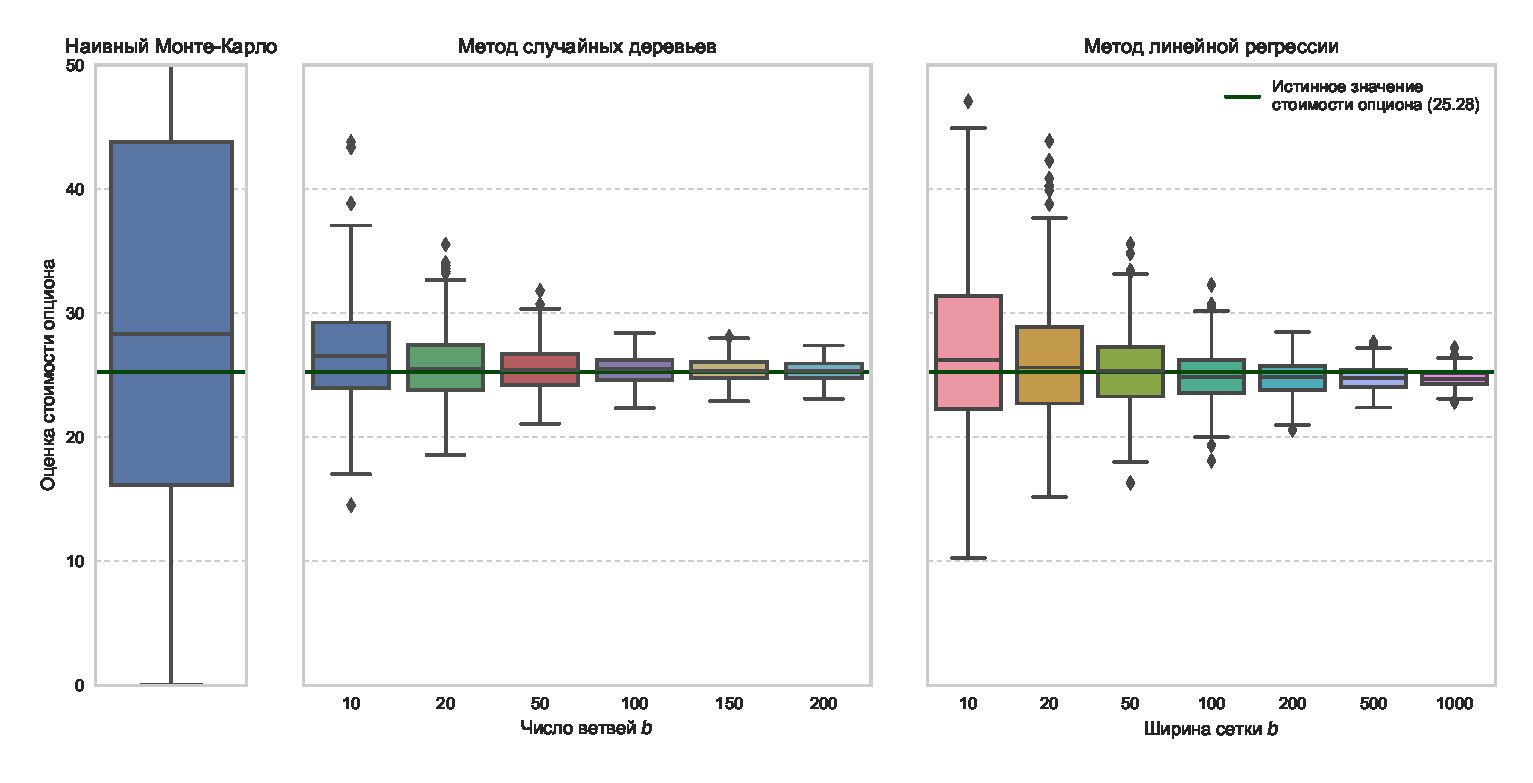
\includegraphics[width=\textwidth]{classical_methods.eps}
%     \caption{Оценки стоимости опциона различными классическими методами}
%     \footnotesize Опцион на 5 независимых базовых активов. Подробное описание параметров моделирования см.~в~секции~\ref{ssub:random_trees_numerical_results}. Результаты метода случайных деревьев описаны в~\ref{ssub:random_trees_numerical_results}, метода наименьших квадратов --- в секции~\ref{ssub:lsm_numerical_results}.
%     \label{fig:classical_methods}
% \end{figure}

% \subsection{Случайные деревья} % (fold)
% \label{sub:tree_estimator}

% Метод случайного дерева основан на моделировании цепи $X_0, X_1, \ldots X_n$ состояний актива. Зафиксируем параметр ветвления $b$. Из исходного состояния $X_0$ смоделируем $b$ независимых следующих состояний $X_1^1, X_1^2, \ldots X_1^b$, все с условием $X_0$. Для каждого $X_1^i$ снова смоделируем $b$ независимых последующих состояний $X_2^{i1}, \ldots X_2^{ib}$. На $m$-ом шаге будем иметь $b^m$ состояний, и это и есть источник основного недостатка этого метода --- его экспоненциальной алгоритмической сложности. Схема приведена на рис.,\ref{fig:exponential_tree}.
% \begin{figure}[b]
%     \centering
%     \includegraphics{exponential_tree.pdf}
%     \caption{Случайное дерево для $b = 3$ и $m = 2$}
%     \label{fig:exponential_tree}
% \end{figure}

% В \cite{Broadie1997} предложены оценки сверху и снизу $\hat{V}_0$ и $\hat{v}_0$ и доказана их состоятельность и асимптотическая несмещённость для $V_0\left(X_0\right)$.
% \begin{equation}\label{eq:upper}
% \begin{aligned}
%     \hat{V}_m^{j_1 \ldots j_m} &= h_m\left(X_m^{j_1 \ldots j_m}\right), \\
%     \hat{V}_i^{j_1 \ldots j_i} &= \max \left\lbrace h_i \left( X_i^{j_1 \ldots j_i} \right), \frac{1}{b} \sum_{j = 1}^b \hat{V}_{i+1}^{j_1 \ldots j_i j}\right\rbrace,
% \end{aligned}\end{equation}
% \begin{equation}\label{eq:lower}
% \begin{aligned}
%     \hat{v}_m^{j_1 j_2 \cdots j_m} &= h\left( X_m^{j_1 j_2 \cdots j_m}\right), \\
%     \hat{v}_{ik}^{j_1 j_2 \cdots j_i} &= \left\lbrace
%                 \begin{array}{l l}
%                     h\left( X_i^{j_1 j_2 \cdots j_i}\right), & \, \text{если } \frac{1}{b-1}\sum_{j=1, j\not= k}^b \hat{v}_{i+1}^{j_1 j_2 \cdots j_i j} \leq h\left(X_i^{j_1 j_2 \cdots j_i}\right), \\
%                     \hat{v}_{i+1}^{j_1 j_2 \cdots j_i k}, & \, \text{иначе}
%                 \end{array}\right. \\
%     \hat{v}_i^{j_1 j_2 \cdots j_i} &= \frac{1}{b}\sum_{k=1}^b \hat{v}_{ik}^{j_1 j_2 \cdots j_i}.
% \end{aligned}\end{equation}

% Алгоритм прост в реализации и нетребователен по памяти: при реализации обходом в глубину память ограничена $O(m)$. Основной недостаток -- экспоненциальная сложность по времени: обойти всё дерево получится за $O(m^b)$.

% \subsubsection{Численные результаты} % (fold)
% \label{ssub:random_trees_numerical_results}

% Для большинства упомянутых в работе методов представлены численные результаты. Алгоритмы были реализованы на языке Python с использованием библиотек NumPy и SciPy~\cite{Jones2001}.

% Результаты работы всех реализованных алгоритмов приведены для одного примера: опцион на покупку на максимум из 5 независимых активов, выписанный на $T = 3$ года, который можно исполнить 4 раза в течение этого срока: в момент получения 0, $T/ 3$, $2T / 3$ и в момент окончания срока действия $T$. Платёжная функция опциона $$h_t(X_t) = \left(\max(X_t) - K\right)^+, X_t\in \mathbb R^5.$$
% Стартовая цена каждого из активов $S_0 = 100$, цена страйк $K = 100$. Поведение опциона моделируется с помощью геометрического броуновского движения (подробное объяснение есть в \cite[стр.~1336]{Broadie1997}), безрисковая процентная ставка $r = 5\%$, дивидендная ставка $\delta = 10\%$ и волатильность стоимости актива $\sigma = 20\%$.

% Это более содержательный пример, чем одномерные опционы, на нём видны некоторые проблемы, которые для одномерных опционов просто не существуют (например, становится нетривиальной задачей разбиение пространства состояний базового актива на ячейки одинаковой вероятности\footnote{Такой вариант понижения вычислительной сложности метода случайных деревьев рассматривался автором, но содержательных результатов для многомерного случая получить не удалось.}). Для этого примера можно найти референсные значения в опубликованных работах (\cite[стр.~57]{Broadie2004}~--~для указанных выше параметров, \cite[табл.~5, стр.~1340]{Broadie1997}~--~для~$T=1$).

% Для метода случайных деревьев была вычислена оценка сверху на стоимость опциона $\Vhat_0$ \eqref{eq:upper}. Результаты представлены на рис.,\ref{fig:classical_methods} и в табл.~\ref{tbl:random_tree_estimators}. Результаты в таблице посчитаны по 500 испытаниям. Если обозначить результат $i$-го испытания за $\Vhat_i$, $n=500$, то обозначения в таблице расшифровываются следующим образом:
% \begin{equation}\label{eq:table_labels}
% \begin{aligned}
% \Vhat &= \frac{1}{n}\sum_{i=1}^n \Vhat_i \\
% \mathrm{sd}\Vhat &= \sqrt{\frac{1}{n}\sum_{i=1}^n \left(\Vhat_i - \Vhat\right)^2} \\
% \mathrm{se}\Vhat &= \sqrt{\frac{1}{n}\sum_{i=1}^n \left(\Vhat_i - V\right)^2} \\
% \mathrm{bias}\Vhat &= \Vhat - V.
% \end{aligned}
% \end{equation}
% Здесь $V$ --- истинное значение стоимости опциона. Для рассматриваемого примера $V = 25.28$, значение взято из \cite{Broadie2004}.

% \begin{table}
%     % \renewcommand{\arraystretch}{0.75}
%     \centering
%     \caption{Оценки методом случайных деревьев}
%     \begin{tabular}{rrrrr}
%         $b$&$\Vhat$&$\mathrm{sd}\Vhat$&$\mathrm{se}\Vhat$&$\mathrm{bias}\Vhat$\\\hline
%         10&26.691&4.145&4.378&1.991\\
%         20&25.690&2.743&2.774&0.168\\
%         50&25.499&1.830&1.843&0.048\\
%         100&25.419&1.163&1.171&0.019\\
%         150&25.379&0.929&0.935&0.010\\
%         200&25.273&0.891&0.892&0.000\\
%     \end{tabular}
%     \label{tbl:random_tree_estimators}

%     \footnotesize
%     Результаты приведены для числа ветвей $b = 10, 20, 50, 100, 150, 200$.\\\vspace{-0.3\baselineskip}Расшифровку обозначений см. в выражении~\eqref{eq:table_labels}.
% \end{table}

% % subsubsection random_trees_numerical_results (end)

% % subsection tree_estimator (end)

% \subsection{Стохастические сетки} % (fold)
% \label{sub:mesh_estimator}

% Метод стохастической сетки также предлагает оценки сверху и снизу для решения \eqref{eq:option-recursive}, но принцип построения оценок несколько отличается от рассмотренного выше метода случайного дерева.

% Из начального состояния $X_0$ для оценки опциона с $m$ моментами исполнения, равноотстоящими во времени от 0 до $T$, зададим сетку $X_n^i, n\in 1\mathbin{:}m, i \in 1\mathbin{:}b$, узлы которой --- реализации случайной величины с плотностью $p_{0, n}(X_0, \cdot)$ (маргинальные плотности; также рассматриваются средние плотности), а $p_{k, n}(x, y) = \prob{X_n = y \middle\vert X_k = x}$. Тогда определяется $\rho_{n, j}(x, y) = p_{n-1, n}(x, y) / p_{0, n}(X_0, y)$, сокращённые обозначения $\rho_{n, j}(i, j) = \rho_{n, j}(X_{n-1}^i, X_n^j)$ и оценка в каждом узле сетки
% $$\hat Y_n(i) = \max\left\lbrace h_n(i), \frac{\sum_j \rho_{n+1}(i, j) \hat Y_{n+1}(j)}{\sum_j \rho_{n+1}(i, j)} \right\rbrace.$$

% Иллюстрация взаимоотношений между узлами сетки приведена на рис.,\ref{fig:stochastic_mesh}. Тогда оценка справедливой стоимости опциона --- это $$\hat Y_0 = \max\left\lbrace h_0(X_0), \frac{\sum_j \rho_{1}(X_0, X_1^j) \hat Y_{1}(X_1^j)}{\sum_j \rho_{1}(X_0, X_1^j)} \right\rbrace.$$

% \begin{figure}[t]
%     \centering
%     \includegraphics{stohastic_mesh_vector.eps}
%     \caption{Стохастическая сетка для $b = 5$ и $m = 3$}
%     \label{fig:stochastic_mesh}
% \end{figure}

% Этот метод работает гораздо быстрее, чем метод случайных деревьев: сложность и по времени, и по памяти составляет $O(mb)$. Недостатком являются трудоёмкие вычисления в многомерном случае: в отличие от случайного дерева, для обсчёта которого нужно лишь уметь вычислить $h_t(X_t)$ (для традиционного примера максимум-опциона на покупку $h_t(X_t) = \left(\max(X_t) - K\right)^+$, если $X_t$ -- вектор стоимостей базовых активов в момент $t$), для стохастических сетей нужно точно вычислять $\rho_n(i, j)$.

% % subsection mesh_estimator (end)

% \subsection{Метод наименьших квадратов} % (fold)
% \label{sub:least_squares}

% Несколько отличающийся от двух предыдущих вариант --- метод оценки с помощью линейной регрессии. Согласно формулировке \eqref{eq:option-recursive}, в каждый момент $t$ мы хотим знать математическое ожидание стоимости удержания (неисполнения) опциона при условии его текущего состояния. Классический инструмент для оценки условного математического ожидания --- это линейная регрессия. Будем оценивать стоимость удержания опциона следующим образом:

% \begin{equation}\label{eq:lsm_continuation}
% \E\left(V_i(X_i)\middle\vert X_{i-1} = x\right) \approx \sum_{r=1}^M \beta_{ir} \psi_r(x) = \beta_i^\mathsf{T}\psi(x).
% \end{equation}
% Здесь $\psi(x) = \left(\psi_1(x), \dots, \psi_M(x)\right)^\mathsf{T}$ --- это набор регрессоров, используемых для построения оценки. В оригинальной статье использовались полиномы Лагера (\cite{Longstaff2001}, секция~2.2 на стр.~122) и для построения регрессии использовались только те траектории, на которых опцион в $i-1$-й момент времени находился в деньгах.

% Мы используем сетку, схожую с той, что была в методе стохастической сетки: моделируем несколько траекторий, тем самым получая нужный набор примеров (см. рис.,\ref{fig:least_squares}). Коэффициенты $\beta$ оцениваются по методу наименьших квадратов. 

% \begin{figure}[t]
%     \centering
%     \includegraphics{stohastic_mesh_vector_phase_0.eps}
%     \caption{Стохастическая сетка для метода наименьших квадратов, $b = 5$ и $m = 3$}
%     \label{fig:least_squares}
% \end{figure}

% Для каждого узла сетки мы можем оценить стоимость удержания опциона по выражению \eqref{eq:lsm_continuation}, и тем самым понять, было ли оптимальным решением исполнить опцион в этот момент. После того, как установлены моменты оптимального исполнения опциона, для каждой из исходных траекторий, составлявших сетку, можно установить стоимость опциона на этой траектории, как выплату, полученную в момент оптимального исполнения. Итоговая стоимость опциона оценивается усреднением по всем траекториям. Более формально эта процедура изложена в алгоритме~\ref{alg:least_squares_estimation}.

% \begin{algorithm}[h]
%     \SetAlgorithmName{Алгоритм}{алгоритм}{Список алгоритмов}
%     \SetKwInput{KwData}{Входные данные}
%     \SetKwInput{KwResult}{Результат}
%     \SetKw{KwTo}{до}\SetKwFor{For}{Для}{\string:}{}%
%     \KwData{сетка из $b$ промоделированных траекторий состояния базового актива $X_n^i, n\in 1\mathbin{:}m, i \in 1\mathbin{:}b$}
%     \KwResult{$\Vhat$ -- оценка стоимости опциона}
    
%     положим стоимость опциона равной выплате по нему в последний момент исполнения:\\$C_i \leftarrow h_{t_m}\left(X_m^i\right)$, $C = \left(C_1, \dots, C_b\right)^{\mathsf T}$\;
%     \For{$n\leftarrow m-1$ \KwTo $1$}{
%         дисконтируем стоимость опциона: $C \leftarrow e^{-r\deltat} \cdot C$\;
%         $X_i \leftarrow S_n^i$, $X = \left(X_1, \dots, X_b\right)^{\mathsf T}$\;
%         выплаты по исполнении опциона $P_i \leftarrow h_{t_n}\left(X_n^i\right)$, $P = \left(P_1, \dots, P_b\right)^{\mathsf T}$\;
%         строим линейную регрессию $C$ на $X$ через набор базисных функций $\psi$ по всем тем примерам, где опцион в деньгах:\\ $\beta \leftarrow \argmin_{\beta'\in\R^M} \norm{\left({\beta'}^\mathsf{T}\psi(X_i) - C_i\right)_{\left\{i \middle\vert P_i > 0\right\}}}^2$\;
%         стоимость удержания опциона $H_i = \beta^\mathsf{T}\psi(X_i)$\;
%         \For{всех $i$ таких, что $P_i > H_i$}{
%             $C_i \leftarrow P_i$\;
%         }
%     }
%     $\Vhat \leftarrow \frac{1}{b}\sum_{i=1}^b C_i$

%     \caption{Оценка стоимости опциона по методу наименьших квадратов}
% \label{alg:least_squares_estimation}
% \end{algorithm}

% В \cite{Glasserman2004} указано, что метод наименьших квадратов можно считать частным случаем метода стохастической сетки со специальным выбором весов. Тем не менее, часто эти подходы рассматриваются по отдельности.

% \subsubsection{Численные результаты} % (fold)
% \label{ssub:lsm_numerical_results}

% Метод наименьших квадратов был реализован для $\psi_1(x) = x, \psi_2(x) = x^2$. Результаты представлены на рис.,\ref{fig:classical_methods} и в табл.~\ref{tbl:lsm_estimators}.

% \begin{table}
%     % \renewcommand{\arraystretch}{0.75}
%     \centering
%     \caption{Оценки методом наименьших квадратов}
%     \begin{tabular}{rrrrr}
%         $b$&$\Vhat$&$\mathrm{sd}\Vhat$&$\mathrm{se}\Vhat$&$\mathrm{bias}\Vhat$\\\hline
%         10&26.870&6.324&6.521&2.527\\
%         20&25.957&4.774&4.822&0.459\\
%         50&25.312&2.877&2.877&0.001\\
%         100&24.965&2.106&2.129&0.099\\
%         200&24.795&1.480&1.557&0.235\\
%         500&24.772&0.918&1.050&0.258\\
%         1000&24.731&0.636&0.840&0.301\\
%     \end{tabular}
%     \label{tbl:lsm_estimators}

%     \footnotesize
%     Результаты приведены для ширины сетки $b = 10, 20, 50, 100, 200, 500, 1000$.\\\vspace{-0.3\baselineskip}Расшифровку обозначений см. в выражении~\eqref{eq:table_labels}.
% \end{table}

% 

% \chapter{Сглаживание случайных деревьев для оценки стоимости Американского опциона} % (fold)
% \label{cha:tree_pruning_for_american_option}

% Метод случайных деревьев, рассмотренный в секции \ref{sub:tree_estimator}, наряду с преимуществами в виде простоты реализации и точности (\textcolor{red}{сравнение точности классических методов за тики}), обладает одним существенным недостатком: из-за экспоненциальной сложности его фактически невозможно использовать для оценки <<настоящих>> Американских опционов, то есть при $m \to \infty$. В этой главе предлагается метод, позволяющий сохранить простоту и точность оценки и при этом использовать случайные деревья для сколь угодно часто исполняемых опционов.

% В некотором смысле предлагаемый метод является комбинацией метода сеток (в частности, метода наименьших квадратов) и метода случайных деревьев. Основная идея заключается в том, что, как только вершин дерева становится слишком много, меняется способ оценки величины $\E\left[V_i\left(X_i\right)|X_{i-1}=x\right]$: вместо рекурсивного построения дальнейшего дерева из точки $x$ используется регрессионная оценка математического ожидания (как в методе наименьших квадратов).

% % chapter tree_pruning_for_american_option (end)

% \appendix

% \chapter{Численные результаты применения квази Монте-Карло к классическим методам} % (fold)
% \label{cha:qmc_numerical_tables}

% Правильные ответы (значения $V$) для примеров из списка \ref{tbl:numerical_examples} взяты из уже опубликованных работ: для примеров 1 и 2 ($\rho=0.3$) из работы, предлагающей метод случайных деревьев \cite{Broadie1997}, для примера 3 из работы, предлагающей метод сеток \cite{Broadie2004}.

% \begin{figure}[p]
%     \centering
%     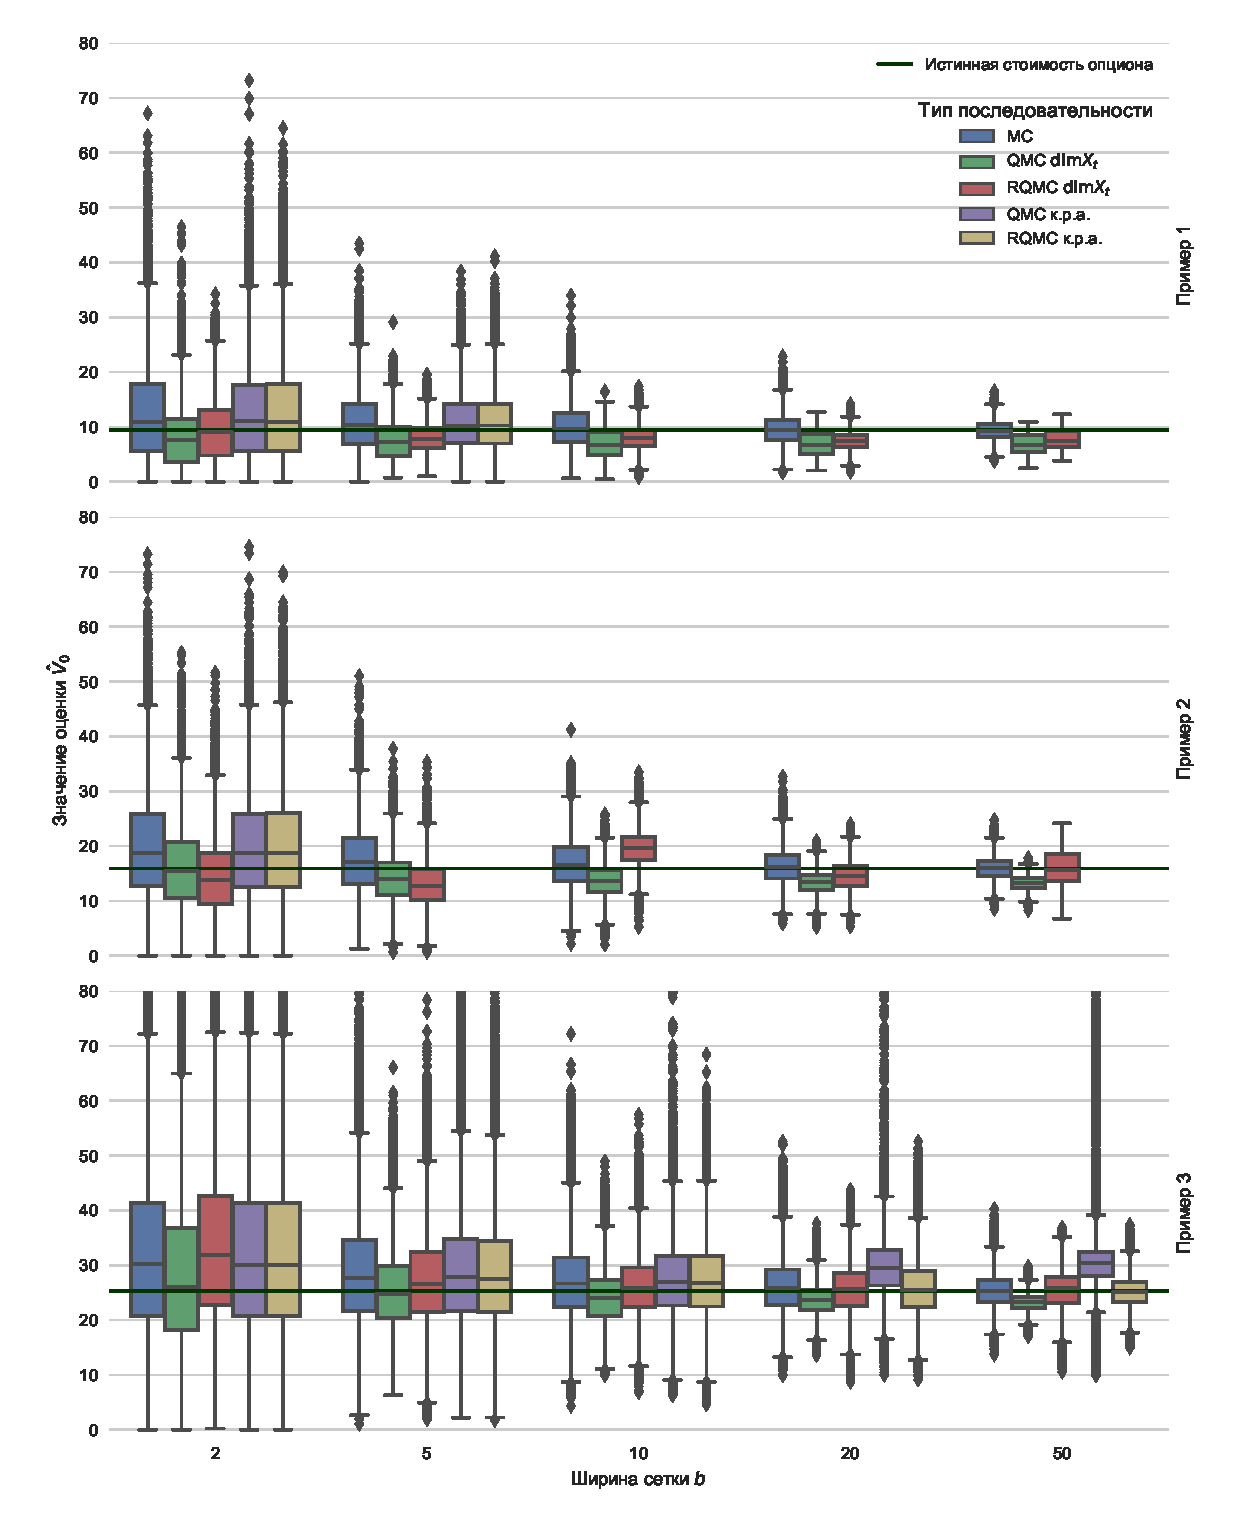
\includegraphics[width=0.9\textwidth]{lsm_sobol.eps}
%     \caption{Разброс оценок стоимости Американского опциона методом наименьших квадратов при использовании псевдослучайных последовательностей (MC) и квазислучайных последовательностей Соболя (QMC) различных размерностей}
%     \label{fig:lsm_sobol}
% \end{figure}

% \begin{table}
%     \renewcommand{\arraystretch}{0.6}
%     \centering
%     Оценки методом наименьших квадратов с псевдослучайной последовательностью (MC) и квазислучайной последовательностью Соболя (QMC)
%     \caption{Пример 1}\label{tbl:lsm_sobol_ex1}
%     \begin{tabular}{rrrrrrr}
%         $b$&тип&$\mathrm{dim} X_t$&$\Vhat$&$\mathrm{sd}\Vhat$&$\mathrm{se}\Vhat$&$\mathrm{bias}\Vhat$\\[3pt]\hline\\[-8pt]
%         2&MC&&12.562&1.856&3.700&3.201\\
%         2&RQMC&12&12.535&1.139&3.372&3.174\\
%         2&RQMC&2&9.516&1.112&1.123&0.155\\[3pt]
%         5&MC&&10.992&1.045&1.937&1.631\\
%         5&RQMC&2&7.938&0.606&1.546&-1.423\\
%         5&RQMC&30&10.957&0.843&1.806&1.596\\[3pt]
%         10&MC&&10.054&0.790&1.051&0.693\\
%         10&RQMC&2&7.893&0.592&1.583&-1.468\\[3pt]
%         20&MC&&9.562&0.501&0.540&0.201\\
%         20&RQMC&2&7.403&0.697&2.078&-1.958\\[3pt]
%         50&MC&&9.306&0.356&0.360&-0.055\\
%         50&RQMC&2&7.673&1.480&2.245&-1.688\\[3pt]
%     \end{tabular}
%     % \footnotesize Пример 1

%     \centering
%     \caption{Пример 2}\label{tbl:lsm_sobol_ex2}
%     \begin{tabular}{rrrrrrr}
%         $b$&тип&$\mathrm{dim} X_t$&$\Vhat$&$\mathrm{sd}\Vhat$&$\mathrm{se}\Vhat$&$\mathrm{bias}\Vhat$\\[3pt]\hline\\[-8pt]
%         2&MC&&19.907&2.077&4.513&4.007\\
%         2&RQMC&30&19.851&1.528&4.236&3.951\\
%         2&RQMC&5&14.446&1.154&1.856&-1.454\\[3pt]
%         5&MC&&17.557&1.270&2.088&1.657\\
%         5&RQMC&5&13.058&1.205&3.087&-2.842\\[3pt]
%         10&MC&&16.819&0.953&1.324&0.919\\
%         10&RQMC&5&19.535&1.231&3.838&3.635\\[3pt]
%         20&MC&&16.353&0.645&0.788&0.453\\
%         20&RQMC&5&14.560&1.754&2.207&-1.340\\[3pt]
%         50&MC&&15.983&0.435&0.443&0.083\\
%         50&RQMC&5&15.958&2.682&2.682&0.058\\[3pt]
%     \end{tabular}
%     % \footnotesize Пример 2

%     \centering
%     \caption{Пример 3}\label{tbl:lsm_sobol_ex3}
%     \begin{tabular}{rrrrrrr}
%         $b$&тип&$\mathrm{dim} X_t$&$\Vhat$&$\mathrm{sd}\Vhat$&$\mathrm{se}\Vhat$&$\mathrm{bias}\Vhat$\\[3pt]\hline\\[-8pt]
%         2&MC&&32.438&3.421&7.934&7.158\\
%         2&RQMC&30&32.285&7.987&10.623&7.005\\
%         2&RQMC&5&35.431&1.825&10.314&10.151\\[3pt]
%         5&MC&&28.570&1.990&3.845&3.290\\
%         5&RQMC&5&25.258&2.010&2.010&-0.022\\[3pt]
%         10&MC&&27.099&1.434&2.316&1.819\\
%         10&RQMC&5&23.328&4.522&4.926&-1.952\\[3pt]
%         20&MC&&26.110&0.941&1.255&0.830\\
%         20&RQMC&5&26.001&0.943&1.187&0.721\\[3pt]
%         50&MC&&25.418&0.605&0.621&0.138\\
%         50&RQMC&5&24.545&2.455&2.563&-0.735\\[3pt]
%     \end{tabular}
%     % \footnotesize Пример 3
% \end{table}

% \begin{figure}[p]
%     \centering
%     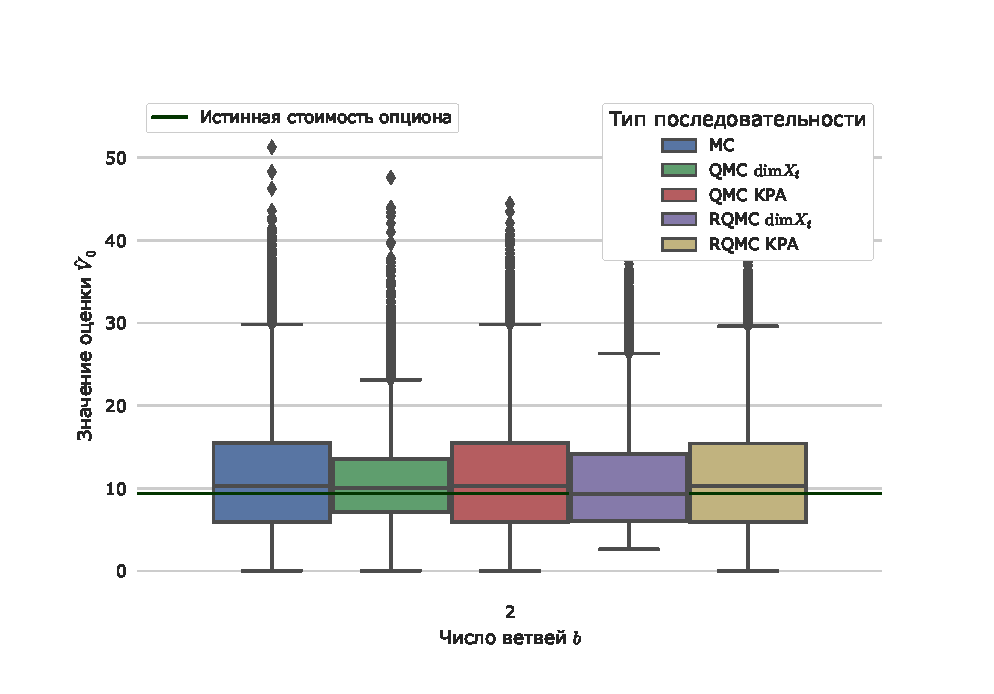
\includegraphics[width=0.9\textwidth]{random_tree_sobol.eps}
%     \caption{Разброс оценок стоимости Американского опциона методом случайных деревьев при использовании псевдослучайных последовательностей (MC) и квазислучайных последовательностей Соболя (QMC) различных размерностей}
%     \label{fig:random_tree_sobol}
% \end{figure}

% \begin{table}
%     \renewcommand{\arraystretch}{0.6}
%     \centering
%     Оценки методом случайных деревьев с псевдослучайной последовательностью (MC) и квазислучайной последовательностью Соболя (QMC)
%     \caption{Пример 1}\label{tbl:random_tree_sobol_ex1}
%     \begin{tabular}{rrrrrrr}
%         $b$&тип&$\mathrm{dim} X_t$&$\Vhat$&$\mathrm{sd}\Vhat$&$\mathrm{se}\Vhat$&$\mathrm{bias}\Vhat$\\[3pt]\hline\\[-8pt]
%         2&MC&&11.232&1.456&2.370&1.871\\
%         2&RQMC&2&10.983&0.638&1.743&1.622\\
%         2&RQMC&28&11.275&0.801&2.075&1.914\\[3pt]
%         5&MC&&10.324&0.762&1.228&0.963\\
%         5&RQMC&2&9.617&0.280&0.380&0.256\\[3pt]
%         10&MC&&9.918&0.448&0.715&0.557\\
%         10&RQMC&2&9.529&0.271&0.319&0.168\\[3pt]
%         20&MC&&9.682&0.333&0.463&0.321\\
%         20&RQMC&2&9.427&0.135&0.150&0.066\\[3pt]
%     \end{tabular}
%     % \footnotesize Пример 1

%     \centering
%     \caption{Пример 2}\label{tbl:random_tree_sobol_ex2}
%     \begin{tabular}{rrrrrrr}
%         $b$&тип&$\mathrm{dim} X_t$&$\Vhat$&$\mathrm{sd}\Vhat$&$\mathrm{se}\Vhat$&$\mathrm{bias}\Vhat$\\[3pt]\hline\\[-8pt]
%         2&MC&&17.934&1.570&2.570&2.034\\
%         2&RQMC&5&19.065&2.004&3.746&3.165\\[3pt]
%         5&MC&&16.990&0.807&1.356&1.090\\
%         5&RQMC&5&17.414&3.428&3.748&1.514\\[3pt]
%         10&MC&&16.499&0.536&0.803&0.599\\
%         10&RQMC&5&18.016&3.273&3.897&2.116\\[3pt]
%     \end{tabular}
%     % \footnotesize Пример 2

%     \centering
%     \caption{Пример 3}\label{tbl:random_tree_sobol_ex3}
%     \begin{tabular}{rrrrrrr}
%         $b$&тип&$\mathrm{dim} X_t$&$\Vhat$&$\mathrm{sd}\Vhat$&$\mathrm{se}\Vhat$&$\mathrm{bias}\Vhat$\\[3pt]\hline\\[-8pt]
%         2&MC&&29.502&2.432&4.873&4.222\\
%         2&RQMC&5&26.231&2.573&2.743&0.951\\[3pt]
%         5&MC&&27.207&1.228&2.285&1.927\\
%         5&RQMC&5&27.666&2.017&3.124&2.386\\[3pt]
%         10&MC&&26.353&0.811&1.346&1.073\\
%         10&RQMC&5&26.673&1.720&2.213&1.393\\[3pt]
%     \end{tabular}
%     % \footnotesize Пример 3
% \end{table}

% \begin{figure}[p]
%     \centering
%     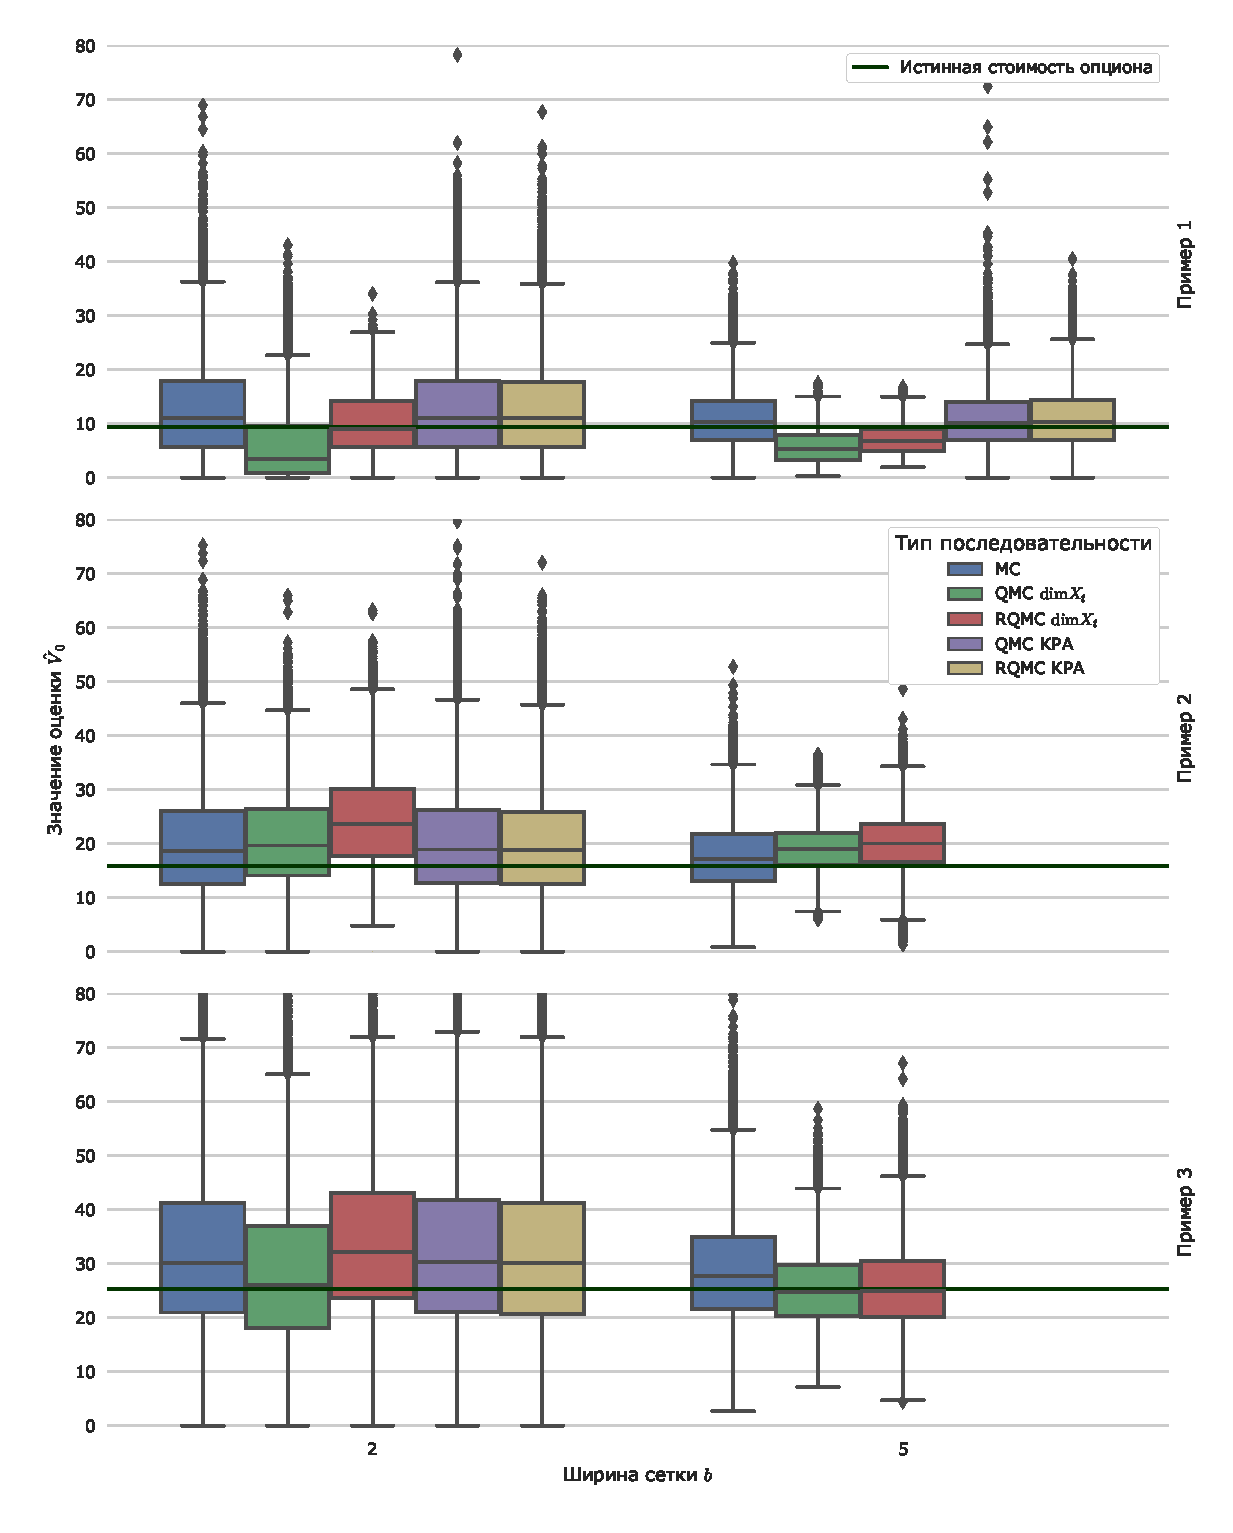
\includegraphics[width=0.9\textwidth]{lsm_halton.eps}
%     \caption{Разброс оценок стоимости Американского опциона методом наименьших квадратов при использовании псевдослучайных последовательностей (MC) и квазислучайных последовательностей Холтона (QMC) различных размерностей}
%     \label{fig:lsm_halton}
% \end{figure}

% \begin{table}
%     \renewcommand{\arraystretch}{0.6}
%     \centering
%     Оценки методом наименьших квадратов с псевдослучайной последовательностью (MC) и квазислучайной последовательностью Холтона (QMC)
%     \caption{Пример 1}\label{tbl:lsm_halton_ex1}
%     \begin{tabular}{rrrrrrr}
%         $b$&тип&$\mathrm{dim} X_t$&$\Vhat$&$\mathrm{sd}\Vhat$&$\mathrm{se}\Vhat$&$\mathrm{bias}\Vhat$\\[3pt]\hline\\[-8pt]
%         2&MC&&12.535&1.818&3.658&3.174\\
%         2&RQMC&12&12.540&2.339&3.947&3.179\\
%         2&RQMC&2&6.119&0.543&3.287&-3.242\\[3pt]
%         5&MC&&10.979&1.094&1.953&1.618\\
%         5&RQMC&2&7.349&0.208&2.023&-2.012\\
%         5&RQMC&30&10.967&2.810&3.237&1.606\\[3pt]
%         10&MC&&10.120&0.736&1.058&0.759\\
%         10&RQMC&2&11.696&0.117&2.338&2.335\\[3pt]
%         20&MC&&9.639&0.549&0.615&0.278\\
%         20&RQMC&2&11.867&0.064&2.507&2.506\\[3pt]
%         50&MC&&9.292&0.348&0.355&-0.069\\
%         50&RQMC&2&7.701&3.284&3.680&-1.660\\[3pt]
%     \end{tabular}

%     \centering
%     \caption{Пример 2}\label{tbl:lsm_halton_ex2}
%     \begin{tabular}{rrrrrrr}
%         $b$&тип&$\mathrm{dim} X_t$&$\Vhat$&$\mathrm{sd}\Vhat$&$\mathrm{se}\Vhat$&$\mathrm{bias}\Vhat$\\[3pt]\hline\\[-8pt]
%         2&MC&&19.753&1.956&4.321&3.853\\
%         2&RQMC&30&19.860&5.361&6.665&3.960\\
%         2&RQMC&5&15.481&0.713&0.827&-0.419\\[3pt]
%         5&MC&&17.478&1.243&2.009&1.578\\
%         5&RQMC&5&19.220&0.622&3.377&3.320\\[3pt]
%         10&MC&&16.822&0.903&1.291&0.922\\
%         10&RQMC&5&15.008&3.358&3.474&-0.892\\[3pt]
%         20&MC&&16.272&0.653&0.751&0.372\\
%         20&RQMC&5&15.612&3.711&3.722&-0.288\\[3pt]
%         50&MC&&16.011&0.429&0.443&0.111\\
%         50&RQMC&5&16.647&3.263&3.348&0.747\\[3pt]
%     \end{tabular}

%     \centering
%     \caption{Пример 3}\label{tbl:lsm_halton_ex3}
%     \begin{tabular}{rrrrrrr}
%         $b$&тип&$\mathrm{dim} X_t$&$\Vhat$&$\mathrm{sd}\Vhat$&$\mathrm{se}\Vhat$&$\mathrm{bias}\Vhat$\\[3pt]\hline\\[-8pt]
%         2&MC&&32.438&3.421&7.934&7.158\\
%         2&RQMC&30&32.285&7.987&10.623&7.005\\
%         2&RQMC&5&35.431&1.825&10.314&10.151\\[3pt]
%         5&MC&&28.570&1.990&3.845&3.290\\
%         5&RQMC&5&25.258&2.010&2.010&-0.022\\[3pt]
%         10&MC&&27.099&1.434&2.316&1.819\\
%         10&RQMC&5&23.328&4.522&4.926&-1.952\\[3pt]
%         20&MC&&26.110&0.941&1.255&0.830\\
%         20&RQMC&5&26.001&0.943&1.187&0.721\\[3pt]
%         50&MC&&25.418&0.605&0.621&0.138\\
%         50&RQMC&5&24.545&2.455&2.563&-0.735\\[3pt]
%     \end{tabular}
% \end{table}

% \begin{figure}[p]
%     \centering
%     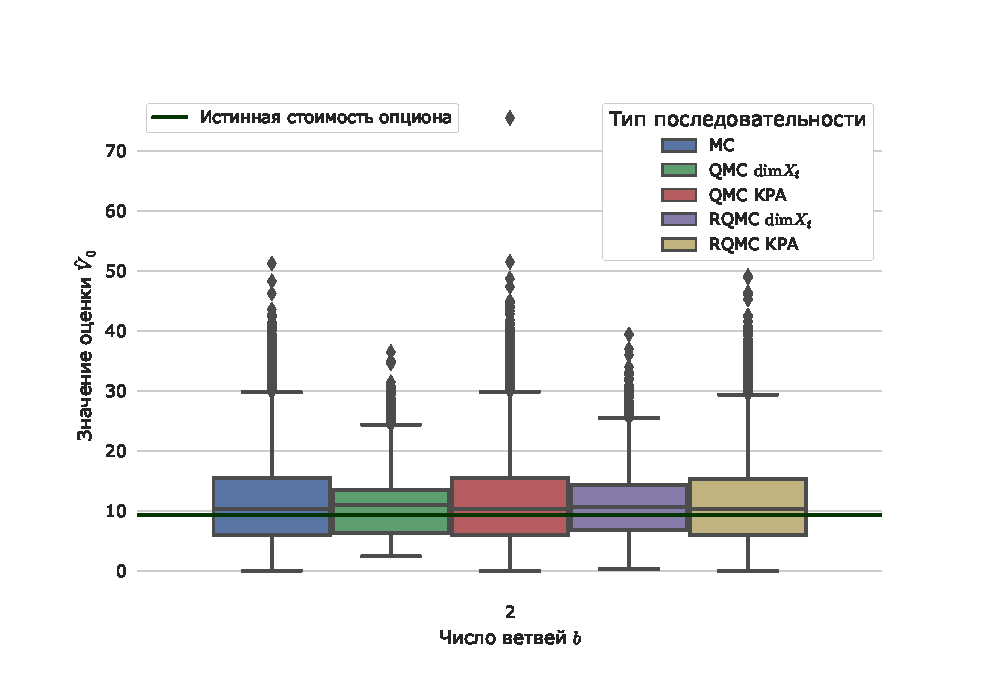
\includegraphics[width=0.9\textwidth]{random_tree_halton.eps}
%     \caption{Разброс оценок стоимости Американского опциона методом случайных деревьев при использовании псевдослучайных последовательностей (MC) и квазислучайных последовательностей Холтона (QMC) различных размерностей}
%     \label{fig:random_tree_halton}
% \end{figure}

% \begin{table}
%     \renewcommand{\arraystretch}{0.6}
%     \centering
%     Оценки методом случайных деревьев с псевдослучайной последовательностью (MC) и квазислучайной последовательностью Холтона (QMC)
%     \caption{Пример 1}\label{tbl:random_tree_halton_ex1}
%     \begin{tabular}{rrrrrrr}
%         $b$&тип&$d$&$\Vhat$&$\mathrm{sd}\Vhat$&$\mathrm{se}\Vhat$&$\mathrm{bias}\Vhat$\\[3pt]\hline\\[-8pt]
%         2&MC&&11.232&1.456&2.370&1.871\\
%         2&RQMC&2&11.014&0.429&1.708&1.653\\
%         2&RQMC&28&11.273&1.969&2.745&1.912\\[3pt]
%         5&MC&&10.324&0.762&1.228&0.963\\
%         5&RQMC&2&9.879&0.217&0.562&0.518\\[3pt]
%         10&MC&&9.918&0.448&0.715&0.557\\
%         10&RQMC&2&9.559&0.465&0.505&0.198\\[3pt]
%         20&MC&&9.682&0.333&0.463&0.321\\
%         20&RQMC&2&9.423&0.110&0.126&0.062\\[3pt]
%     \end{tabular}
%     % \footnotesize Пример 1

%     \centering
%     \caption{Пример 2}\label{tbl:random_tree_halton_ex2}
%     \begin{tabular}{rrrrrrr}
%         $b$&тип&$d$&$\Vhat$&$\mathrm{sd}\Vhat$&$\mathrm{se}\Vhat$&$\mathrm{bias}\Vhat$\\[3pt]\hline\\[-8pt]
%         2&MC&&17.934&1.570&2.570&2.034\\
%         2&RQMC&5&20.616&1.608&4.982&4.716\\[3pt]
%         5&MC&&16.990&0.807&1.356&1.090\\
%         5&RQMC&5&16.666&2.346&2.467&0.766\\[3pt]
%         10&MC&&16.499&0.536&0.803&0.599\\
%         10&RQMC&5&16.919&2.904&3.078&1.019\\[3pt]
%         20&MC&&16.193&0.351&0.458&0.293\\
%         20&RQMC&5&16.510&2.216&2.299&0.610\\[3pt]
%     \end{tabular}
%     % \footnotesize Пример 2

%     \centering
%     \caption{Пример 3}\label{tbl:random_tree_halton_ex3}
%     \begin{tabular}{rrrrrrr}
%         $b$&тип&$d$&$\Vhat$&$\mathrm{sd}\Vhat$&$\mathrm{se}\Vhat$&$\mathrm{bias}\Vhat$\\[3pt]\hline\\[-8pt]
%         2&MC&&29.502&2.432&4.873&4.222\\
%         2&RQMC&5&28.972&2.018&4.208&3.692\\[3pt]
%         5&MC&&27.207&1.228&2.285&1.927\\
%         5&RQMC&5&27.505&1.984&2.981&2.225\\[3pt]
%         10&MC&&26.353&0.811&1.346&1.073\\
%         10&RQMC&5&26.786&1.730&2.293&1.506\\[3pt]
%         20&MC&&25.826&0.533&0.763&0.546\\
%         20&RQMC&5&26.281&1.407&1.727&1.001\\[3pt]
%     \end{tabular}
%     % \footnotesize Пример 3
% \end{table}

% chapter qmc_numerical_tables (end)

\printbibliography[heading=bibintoc]

\end{document}

